\section{Basic findings}
\subsection{Densest CZ have experienced faster decline in the gender wage gap}
Consider the regression
\beqns
	gap_{r2020}-gap_{r1970}=\alpha + \beta\ln(density)_{r1970}
\eeqns
where $gap_r=w_r^{male}-w_r^{female}$, where $w$ stands for average log-wage in the commuting zone.


Table \ref{table:overall_change} shows the estimates of $\beta$ for different average wage measures. All the estimates are significant and negative $\implies$ densest CZ experienced a significantly larger reductions in the gender wage gap. 

\paragraph{Several observations}

%Add a little of perspective in terms of what happens if I move from x cz to y cz.

\bitem 
	\item \textbf{Density measure:} \cite{Duranton2020} argue that total population is more linked to the ``experienced'' density in a labor market than the ``naive'' population density. Table \ref{table:overall_change} shows that the gradient is virtually unchanged when using: ``naive'' CZ population density, or total CZ population.
	\item \textbf{Magnitude of the coefficient:} The gradient is large under multiple benchmarks. Let's focus on interpreting the gradient for the raw wage gap on population density.
	\bitem 
		\item \textbf{Standardized effect} an increase of 1 s.d. in population density (1.18) $\implies$ a change of -.4 s.d.  in the gender wage gap.  A model with just just population density accounts for 17\% of the variation 1970-2020 gender gap change.
		\item \textbf{IC gap:} a CZ in the 25 percentile had an expected decline in the gap of 23 log points. In contrast, a CZ in the 75 percentile experienced a 27 log-point decline $\implies$ a decrease that is 17\% larger.  
		\item \textbf{IC gap relative to the mean:} the 4 log-point gap is equivalent to $15.6\%$ of the decline in the gender gap for \textit{the average CZ}.
	\eitem 	
\eitem 


\begin{figure}[!h]
\centering
\caption{Change in gender wage gap, 1970-2020}
\label{figure:overall_change}
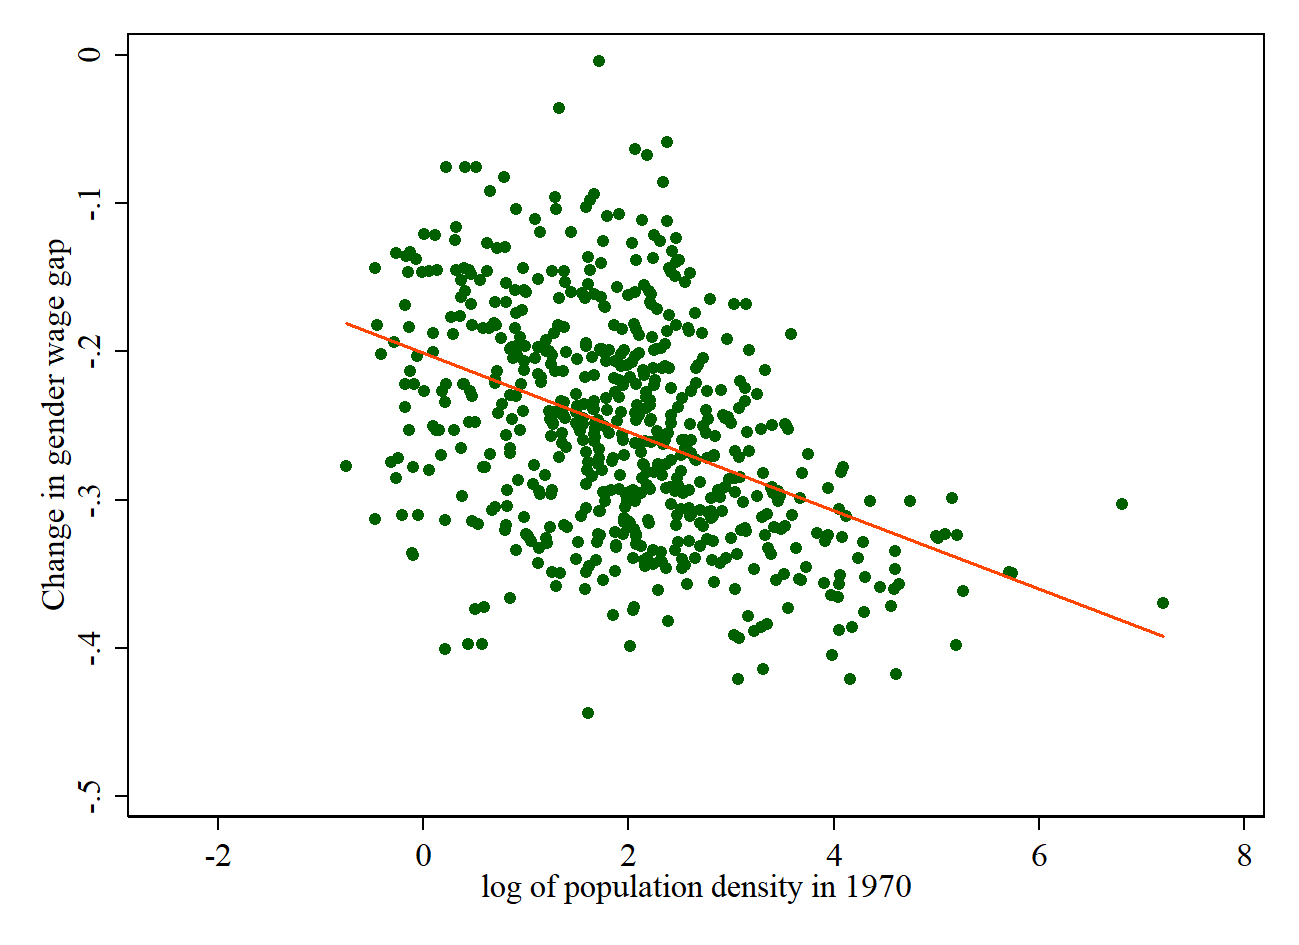
\includegraphics[width=.5\textwidth]{../2_analysis/output/figures/change_1970_2020}
\par \begin{minipage}[h]{\textwidth}{\tiny\textbf{Note:} figure restricts to CZ with more than 1 people per km$^2$. Figure generated on 30 Nov 2020 at 11:17:17. Figure generated using the dofile 2\_analysis/code\_files/write\_regression\_coefplots.do.}\end{minipage}
\end{figure}


\begin{center}
\begin{threeparttable}[!h]
\caption{Gender wage gap vs density}
\label{table:overall_change}
\begin{tabular}{lccc}
\toprule
\toprule
\textbf{}&\multicolumn{1}{c}{\textbf{Raw gap}}&\multicolumn{1}{c}{\textbf{Net of basic controls}}&\multicolumn{1}{c}{\textbf{Net of human capital controls}} \\
\midrule
l\_czone\_density\_70  &      -0.026\sym{***}&      -0.027\sym{***}&      -0.022\sym{***}\\
                    &     (0.002)         &     (0.002)         &     (0.002)         \\
l\_czone\_pop\_70      &      -0.025\sym{***}&      -0.025\sym{***}&      -0.023\sym{***}\\
                    &     (0.002)         &     (0.002)         &     (0.002)         \\
\bottomrule
\bottomrule
\end{tabular}
\begin{tablenotes}
\item \footnotesize \textit{Note:} changes based on unweighted estimated elasticities. Sample restricted to full-time year-round workers. Table generated on 30 Nov 2020 at 11:17:18. Table generated with do file 2\_analysis/code\_files/write\_regression\_coefplots.do
\end{tablenotes}
\end{threeparttable}
\end{center}


\subsection{The relationship between density and gender gap went from positive to negative during 1970-2020}

In figure \ref{figure:baseline_gradients} I show estimates of $\beta_t$ in the regression:
\beqns
	gap_{rt}=\alpha_t+\beta_t\ln(density)_{rt}
\eeqns

\paragraph{Several remarks}
\bitem
	\item The density gradient declined gradually over the period. It went from positive in 1970 to negative in the 2020.
	\item The gradient declines roughly in 2.7 log-points, which roughly corresponds to the coefficient found in in the previous section.
	\item The inversion of the gradient is robust to controlling for basic individual characteristics.
\eitem 
\begin{figure}[!h]
\centering
\caption{Coefficient on population density $ \beta_t $}
\label{figure:baseline_gradients}
\subfloat[Alternative density measures]{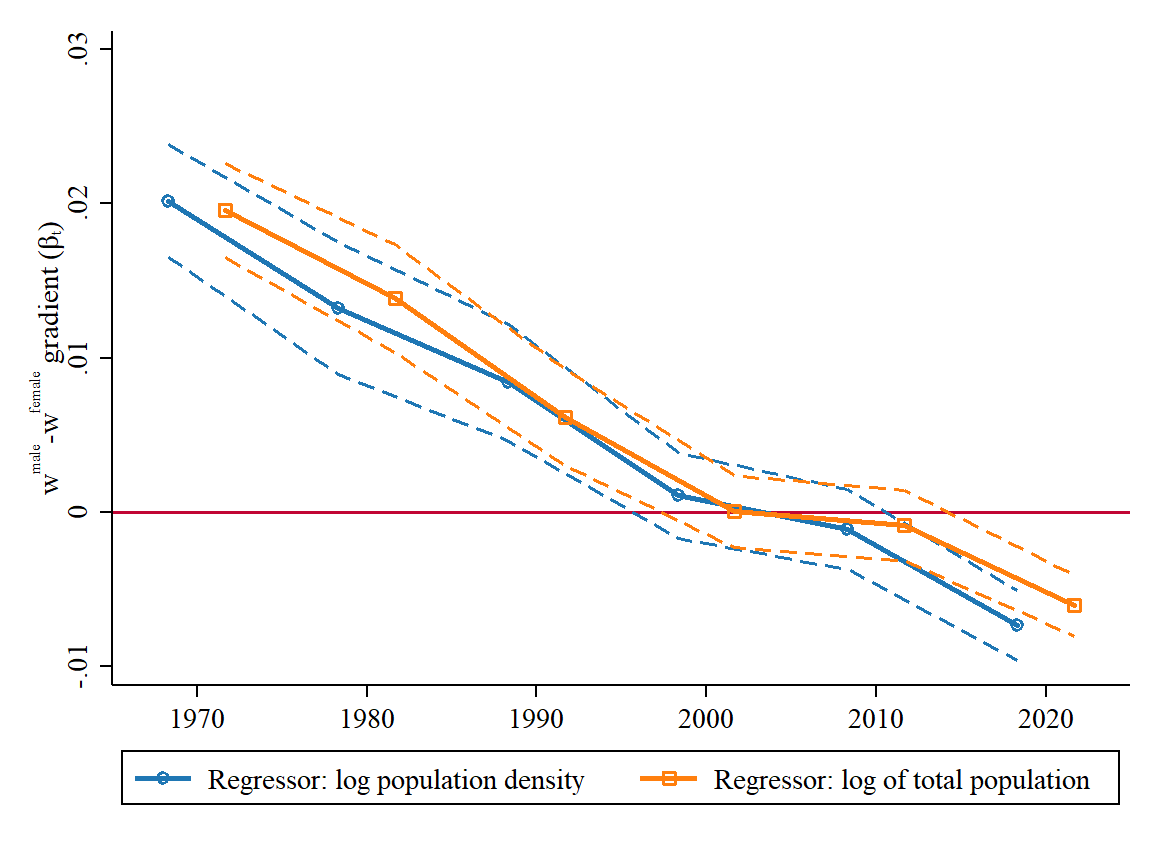
\includegraphics[width=.5\textwidth]{../2_analysis/output/figures/baseline_full_time}} \subfloat[Alternative gender gap measures]{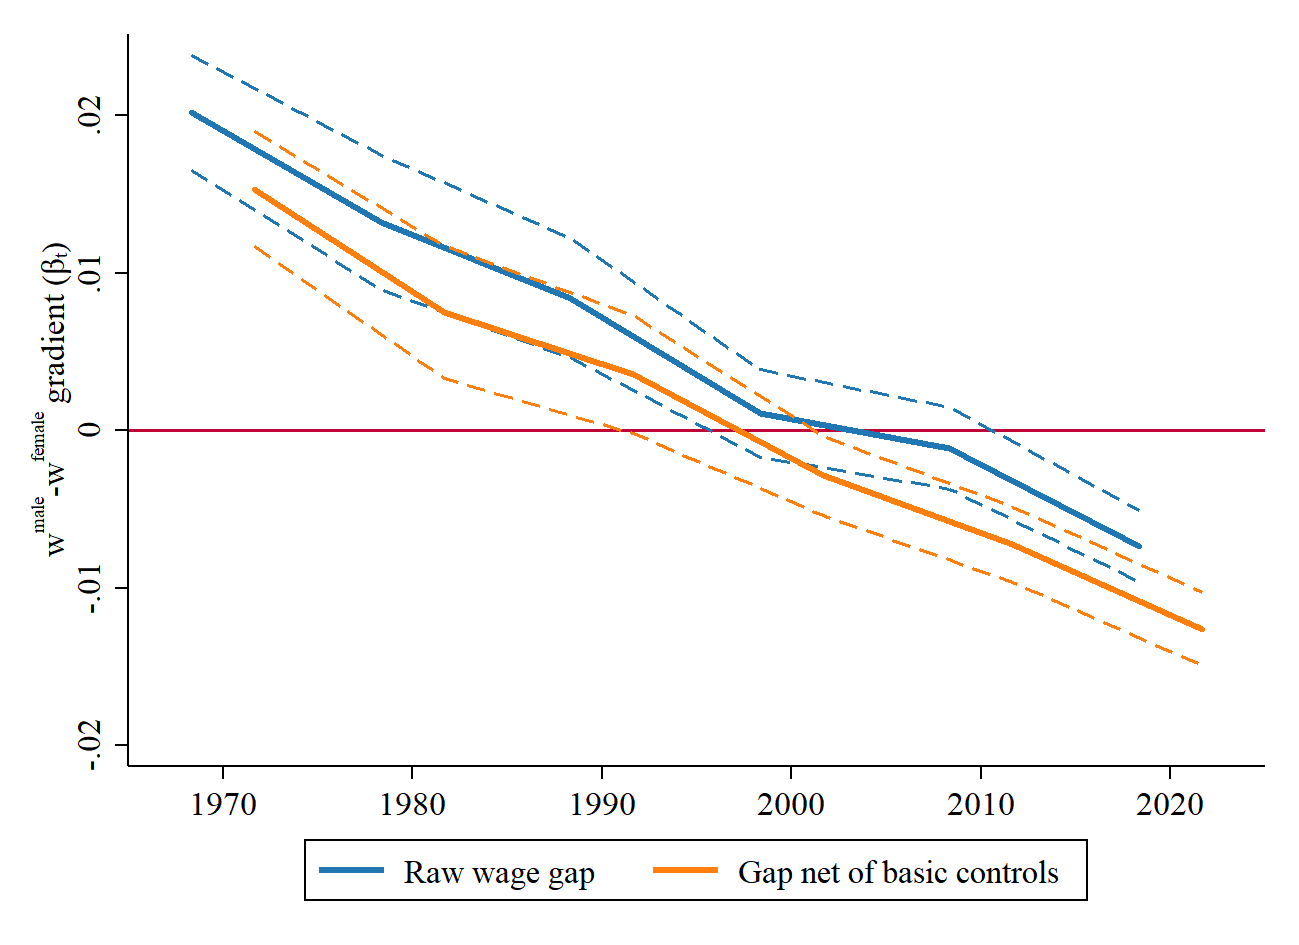
\includegraphics[width=.5\textwidth]{../2_analysis/output/figures/baseline_bas_full_time}} \\ 
\par \begin{minipage}[h]{\textwidth}{\tiny\textbf{Note:} figure restricts to CZ with more than 1 people per km$^2$. Bars show 90\% confidence intervals. Standard errors clustered at the CZ level. Figure generated on 23 Nov 2020 at 16:25:25. Figure generated using the dofile 2\_analysis/code\_files/write\_regression\_coefplots.do.}\end{minipage}
\end{figure}


\paragraph{The cross-sectional gradient in perspective:}
\bitem 
\item \textbf{Implied IC gap}:
\bitem
	\item 1970: 2.8 log-points $\implies$ .4 s.d. increase in gender gap. This is also equivalent to an increase of 7\% in the gender wage gap. 
	\item 2020: 1.16 log-points $\implies$ .3 s.d. increase in gender gap. This is also equivalent to an increase of 6\% in the gender gap. If I account for differences in the age distribution of the population, then this difference becomes 2 log-points. Again, this is roughly equivalent to .2 s.d. in the adjusted wage gap.
\eitem
	\item \textbf{In international perspective:} 
	\bitem 
	\item The US is the 6th country with the highest gender gap within the the OECD. Moving from a 10th percentile CZ to a 90th in 2020 $\implies$ decline of 3 log-points in the gender gap. This is roughly equivalent to moving from the US to Germany $\approx$ erasing 50\% of the gap between the US and the average for OECD countries \href{https://data.oecd.org/earnwage/gender-wage-gap.htm}{see this data}.
	\item \textbf{Tangential remark on gender sd:} there is as much variation in the gender gap within the US (2020), as there is in the across countries in the OECD.

\eitem
\item \textbf{In terms of the urban wage premium?}
\bitem 
	\item \textbf{In 2020}: the urban wage premium for men was of 4.4 log points. For women was 5.2 log-points $\implies$ 18\% larger premium for women. Adjusting wages for age / race $\implies$ premium for women was 25\% larger than for men.
	\item \textbf{Change across time:} since the peak in 1990, male's premium declined by 3.84 log-points 47\% (41\% when adjusting by age / race). By comparison, women's premium declined by 2.25 log points. This a decline of 30\% (26\% when adjusted by age / race) $\implies$ this is a big difference in the evolution of men's and women's fortunes. Women's decline in the premium is just 58\% of men's decline in the premium.
\eitem
My conclusion here, is that the observed coefficients on density are big relative to the overall within-country variation in the gender gap, even though the IC seems modest.
\eitem

\subsection{Further checks}
\subsubsection{Is the density gradient just capturing cross-region variation?} No. The gradient and it drift is robust to controlling for region and state fixed effects!

\begin{figure}[!h]
\centering
\caption{Density gradient is robust to adding region and state fixed-effects}
\label{figure:baseline_gradients}
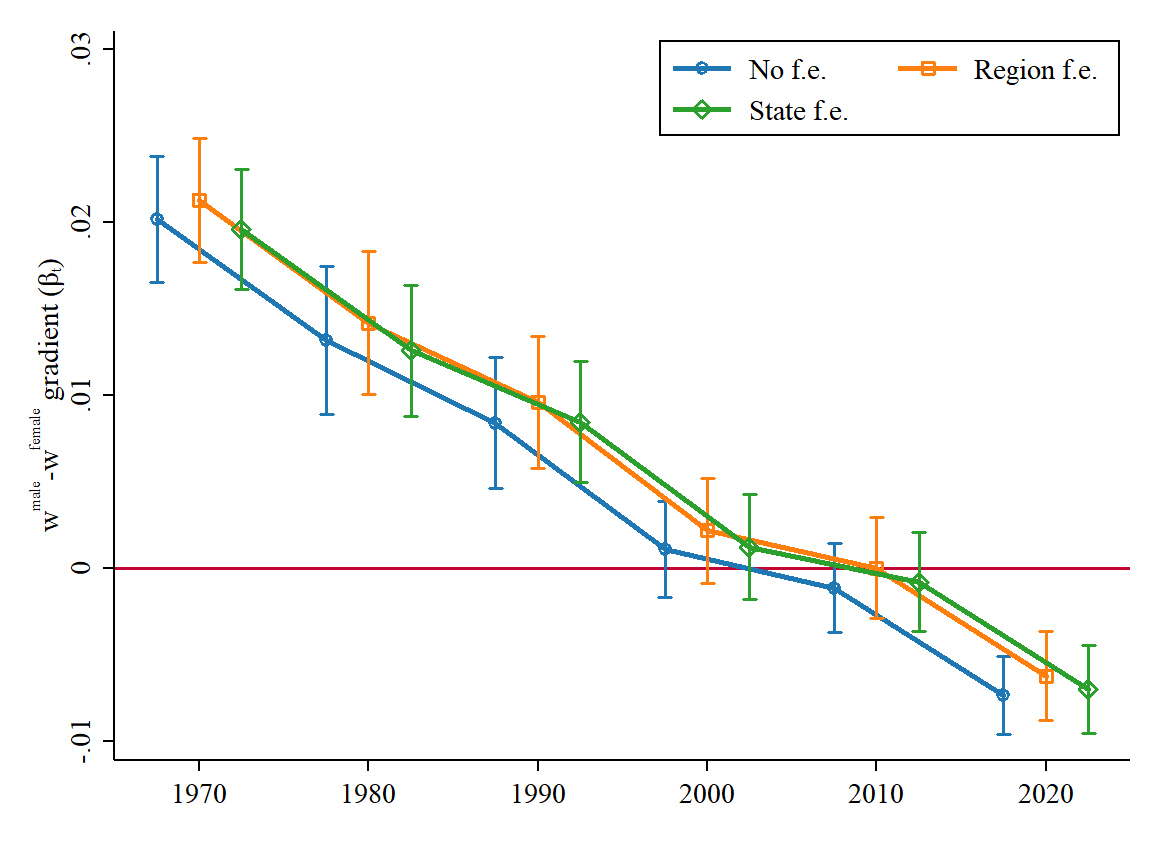
\includegraphics[width=1\textwidth]{../2_analysis/output/figures/region_fe_full_time.png}
\par \begin{minipage}[h]{\textwidth}{\tiny\textbf{Note:} figure restricts to CZ with more than 1 people per km$^2$. Bars show 90\% confidence intervals. Standard errors clustered at the CZ level. Figure generated on 30 Nov 2020 at 11:17:20. Figure generated using the dofile 2\_analysis/code\_files/write\_regression\_coefplots.do.}\end{minipage}
\end{figure}



\subsubsection{The drift in the gradient is not driven just by small / rural CZ}

One concern with the results in the previous sections is that they might be driven by very small CZ, which are relatively unpopulated and which have little bearing in the overall US labor market. To study whether this is a concern I also compute gradients for ``big'' CZ.  I define big CZ as those which had a population density of at least 2.5 people per km$^2$ in 1950. These 175 CZs had a median population of 316k people and accounted for around 74\% of the US population in all the years I am considering. 



Figure \ref{fig:big_CZ} shows that this is not the case. There I compare the gradients for all CZ vs those I get when I limit estimation to big CZ only. Two features stand out:
\benu
	\item The gradient \textit{also arises for the} the largest CZ.
	\item Big CZ also feature a decline in the gender-gap gradient. However, this decline is concentrated on the 1970-1990 period. From then on, the gradient remains negative and roughly constant. Panel (b) shows that the picture remains unchanged if I adjust wages for age / race.
\eenu

%can I explain this with just the changes in the industrial structure?

\begin{block}{Takeway from this exercise:}
	The gender gap gradient is not driven just by small CZ. Big CZ feature a more striking pattern of gradient decline during 1970-1990. Smaller CZ do drive the gradual decline from 1990 onward.
\end{block}

\input{../2_analysis/output/figures/big_cz_full_time.tex}

\subsubsection{Is this about gender?}

Given the facts shown above, a natural question to ask is whether this is really about gender? In other words, do I see similar patterns when, for instance, I examine race? To test this I perform a similar exercise for the black-white gap. I run the regression,
\beqns
	w^{white}_{rt}-w^{black}_{rt}=\alpha_t+\beta_t\ln(density)_{rt}
\eeqns
Figure \ref{fig:race_gradient} shows the estimated $\beta_t$. The decline in the gradient does not appear in race. In fact, with the exception of 1990, there is little change in the gradient over the whole period.

\begin{block}{Takeaway}
 There is something distinct between the interaction of gender and population density
\end{block}

\begin{figure}[!h]
\centering
\caption{Coefficient on population density $ \beta_t $}
\label{fig:race_gradient}
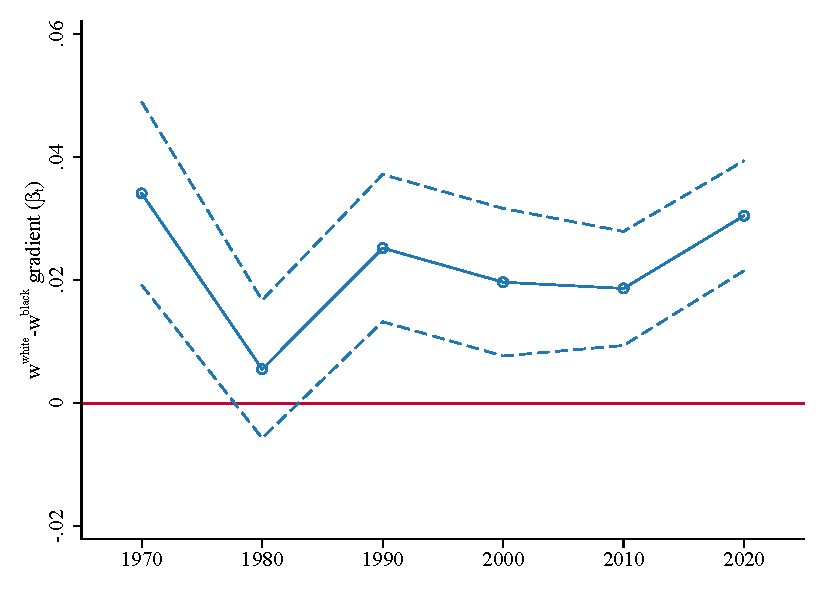
\includegraphics[width=.6\textwidth]{../2_analysis/output/figures/baseline_race_gradients_l_czone_density_full_time}
\par \begin{minipage}[h]{\textwidth}{\tiny\textbf{Note:} figure restricts to CZ with more than 1 people per km$^2$. Bars show 90\% confidence intervals. Standard errors clustered at the CZ level. The figure restricts to year-round full time men workers. Figure generated on 30 Nov 2020 at 11:17:27. Figure generated using the dofile 2\_analysis/code\_files/write\_regression\_coefplots.do.}\end{minipage}
\end{figure}

 
\section{Questions inspired by these facts?}
\bitem
	\item Why has the decline in the urban premium has been less severe for women over the period?
	\item What explains the inversion in the gender gap - density gradient?
	\item Do women benefit more from moving to a city today?
\eitem


\subsection{Incipient answers}
\subsubsection{Do women benefit more from cities?}
\paragraph{Fixing ideas}
To fix ideas let's consider the following model for wages, where $g$ indexes gender and $r$ indexes region:
\beqns
	w_{iert}^g=\alpha_t+\delta_{et}+\gamma_{ert}^g+\varepsilon_{it}
\eeqns
For the sake of the argument, suppose $e$ indexes education. Here $\delta_e$ represents the economy-wide return to having education $e$, while $\gamma$ represents the region-specific return to education. Then, the average wage in a commuting zone is given by,
\beqns
		w_{rt}^g=\alpha_t+\sum_es_{ert}^g\delta_{et}+\sum_es_{ert}\gamma_{ert}+u_{rt}
\eeqns
To fix ideas, let us impose the strong assumption that $\gamma_{ert}=\omega^g_t\ln(density)_{rt}+\nu_{rt}$ the above equation reduces to:
\beqns
	w_{rt}^g=\alpha_t+\sum_es_{ert}^g\delta_{et}+\omega^g_t\ln(density)_{rt}+v_{rt}
\eeqns
By running the regression:
\beqns
	w_{rt}^g=\alpha+\beta^g_t\ln(density)_{rt}
\eeqns
we have that:
\beqns
	plim(\beta^g_t)=\omega^g_t+\frac{cov(\sum_es_{ert}^g\delta_{et},\ln(density)_{rt})}{var(\ln(density)_{rt})}
\eeqns
therefore $\beta^g_t$ has two components
\bitem
	\item $\omega^g_t=$ gender-specific urban wage premium.
	\item A term reflecting bias due to heterogeneous composition of the population across labor markets. For example, if high-wage groups are more likely to locate in cites $\implies$ $\beta^g_t$ overestimates the gains from moving to a city.
\eitem
I will impose another strong assumption. Let $\frac{cov(\sum_es_{ert}\delta_{et},\ln(density))}{var(\ln(density)_{rt})}=\chi^g_t$.

Then, abusing a bit of notation, we have
\beqns
	\beta^g_t=\omega^g_t+\chi^g_t
\eeqns
This simple model suggests a procedure to decompose the density gradient into the selection / urban premium components.
\benu
	\item $\beta_t^g$ is obtained from a simple regression of average \textit{raw wages} on population density.
	\item Under the assumption of $\gamma_{ert}=\omega^g_t\ln(density)_{rt}$ an individual's wage is reduced to:
	\beqns
		w^g_{iert}=\alpha_t+\delta_{et}+\gamma_{rt}^g+\varepsilon_i
	\eeqns
	which is just a regression of individual's wages on education fixed-effects, and a gender$\times$CZ fixed effects. In this case $\gamma_{rt	}^g$ gives an estimate of $\omega^g_t\ln(density)_{rt}$.
	\item From there, it is straightforward to obtain an estimate of the urban wage premium, just estimate the regression:
	\beqns
		\gamma^g_{rt}=\eta_t + \omega_t^g ln(density)_{rt}+\nu_{rt}
	\eeqns 
	\item The selection component is obtained out of the difference between the estimates in part 1 and 3.
\eenu
\subparagraph{Some remarks:}
\bitem 
	\item In the discussion above I am assuming that the urban wage premium is the same for education groups $\gamma_{er}^g=\omega^g_t\ln(density)_{rt}$. If the premium were education-specific then,
	\beqns
		w_{rt}^g=\alpha_t+\sum_es_{ert}^g\delta_{et}+\sum_es_{ert}\omega^g_{et}\ln(density)_{ert}+u_{rt}
	\eeqns
	which would introduce heterogeneity in the density gradient across commuting zones. One can easily explore whether this is an issue by estimating $\omega^g$ by education group (this is feasible only when there is a limited number of education groups).
\eitem 

\paragraph{Results}
\subparagraph{Premium today:} in the table below I show the decomposition described above under different sets of controls.

\addfig{.75}{../2_analysis/output/tables/decomposition_premium_2020}

\textbf{Interpretation notes:}
\bitem
	\item From left to right, each column adds a new set of regressors controls. Thus the interpretation of the selection component in, say the human capital column, is how much of the density gradient is accounted by the human capital controls, over an above the basic set of controls. As a result, the $\%$ explained column is computed relative to the adjusted premium in the basic column.
	\item A negative selection component $\implies$ denser cities have higher shares of low wage groups.
	\item A positive component $\implies$ denser cities have lower shares of low income groups.
\eitem
\textbf{What does stand out?}
\bitem
	\item Women's premium is always larger than men's.
	\item Selection component of basic (age, rage, foreign born dummies) is always negative (city's population is blacker and younger, which tend to be associated with a lower income). \textit{Selection on basic demographics} is twice as important for women than for men.
	\item Selection on education, industry, occupation is very similar for both genders.
	\item \textbf{Overall message:} even after accounting for this rich set of characteristics, women's premium is positive and bigger than men. Cities appear to draw more women from low-wage groups $\implies$ accounting for different demographic composition actually \textit{increases} women's relative density premium.
\eitem
\subparagraph{Premium over time}
The table below shows the decomposition of the density gradient for three selected years. \newline
\textbf{What does stand out?}
\bitem 
	\item In 1970, city women were more likely to come from low education groups. This had reversed by 2020.
	\item 1970-1990: Accounting for industry of employment eliminates the gender gap in the urban premium. Even though both genders are employed in higher pay industries in cities, men are more likely to do so $\implies$ most of density premium can be explained by gender segregation across industries.
	\item Note however, that industry and occupation does not erase the gap in the urban premium across genders in 2020. Even after accounting for industry and employment, the women's premium is 56\% larger than men's.
	\item The table also makes clear the pattern already noted by [cite autor here]. There's a precipitous decline in men's urban wage premium. If we concentrated in the last column, between 1990 and 2020 men's premium declines by 61\%. What is remarkable, is that women's premium is relatively more resilient, declining by 40\% over the same period.
	\item Without adjusting for industry and occupation men's decline in the premium was so strong that it went from being \textit{above} women's, to being below it.
\eitem 

The attached coefficient plots basically paint the same picture. They also suggests that the reversal of fortunes happened during the 1990s. From then on, there is a gradual expansion of the gender gap in the premium.

\begin{figure}[!h]
\centering
\caption{Coefficient on population density $ \beta_t $ controlling for worker characteristics}
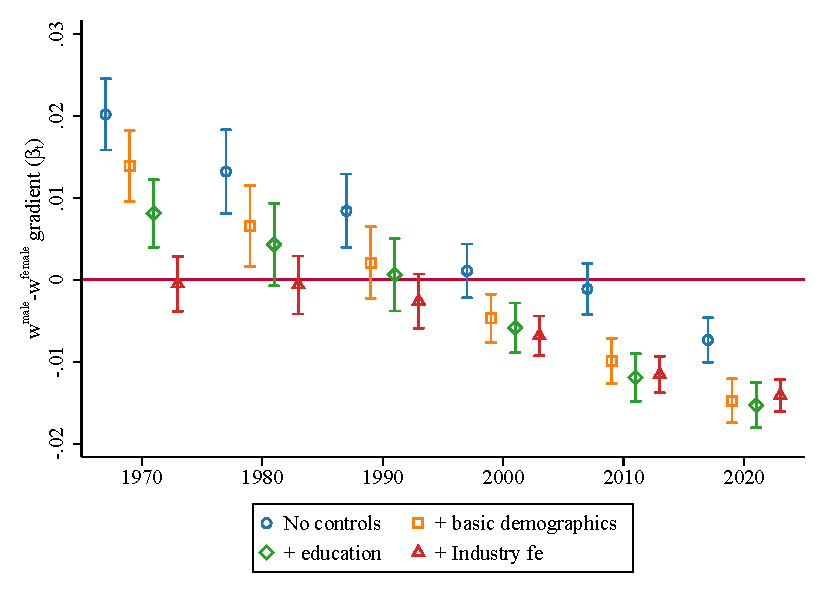
\includegraphics[width=.6\textwidth]{../2_analysis/output/figures/with_control_gradients_individual_l_czone_density_full_time}
\par \begin{minipage}[h]{\textwidth}{\tiny\textbf{Note:} figure restricts to CZ with more than 1 people per km$^2$. The regressions are done on data aggregated at the CZ level after residualizing individual-level characteristics. Bars show 95\% confidence intervals. Errors clustered at the CZ-level.}\end{minipage}
\end{figure}




\paragraph{Some interpretation caveats}
\bitem
	\item In the discussion above I am interpreting  $\hat{\omega}^m_t-\hat{\omega}^f_t$ as evidence of differneces genders in the urban wage premium. This interpretation might not be correct. For example, suppose that urban wage premium differs by education level, but not across genders. That is:
	\beqns
		\gamma_{ert}^m=\gamma_{ert}^f=\omega_{et}\ln(density)_{er}
	\eeqns
	note that in this case:
	\beqns
		w_{rt}^m-w_{rt}^f=\alpha^m_t-\alpha^f_t+\sum_e\delta_e(s_{ert}^m-s_{ert}^f)+\sum_{e}\omega_{et}(s_{ert}^m-s_{ert}^f)\ln(density)_{rt}+u_{rt}
	\eeqns
	Under this scenario the gradient on density is given by:
	\beqns
		\sum_{e}\omega_{et}(s_{ert}^m-s_{ert}^f)
	\eeqns
	The expression above will likely be negative if:
	\bitem 
		\item Women concentrate more heavily in high urban wage premium groups.
	\eitem 
	If we now focus on the drift down of the premium, men's advantage will decline if:
	\bitem
		\item The premium for men-heavy groups is declining over time.
		\item Or women are increasingly concentrating in high urban premium groups.
	\eitem
	Note that this model also suggests' a quick way to discard this possibility. Note that the within-group gender wage wage is given by:
	\beqns
			w_{ert}^m-w_{ert}^f=\alpha^m_t-\alpha^f_t+u_{rt}
	\eeqns
	thus there shouldn't be a within-group gender-gap gradient on density. Given the increase in women's educational attainment since the 1970 education is a natural target to apply this test.
	
	The discussion above takes the proposed model too seriously, but it gives an useful intuition. If the drift in the gender-gap premium is driven by differences in group premia + changes in the the composition of the labor force across genders, then these issues should be less prevalent when I compute the regressions by group.
\eitem 

\addfig{.75}{../2_analysis/output/tables/decomposition_1990_2020}

\subsection{Are the results above driven by different wage premium across educational groups?}

\noindent\textbf{Short answer}: no. But the drift in the gender-gap gradient is driven by workers without a bachelor degree.

Panel a in figure \ref{figure:education_shares} shows that women educational attainment have increased dramatically relative to men. Panel b shows that it has increased more in the densest labor markets. If the urban wage premium of college graduates is larger than non-college graduates, then this trends could drive the patterns described in previous sections.


\begin{figure}[!h]
\centering
\caption{Educational attainment by gender}
\label{figure:education_shares}
\subfloat[Average share college graduates]{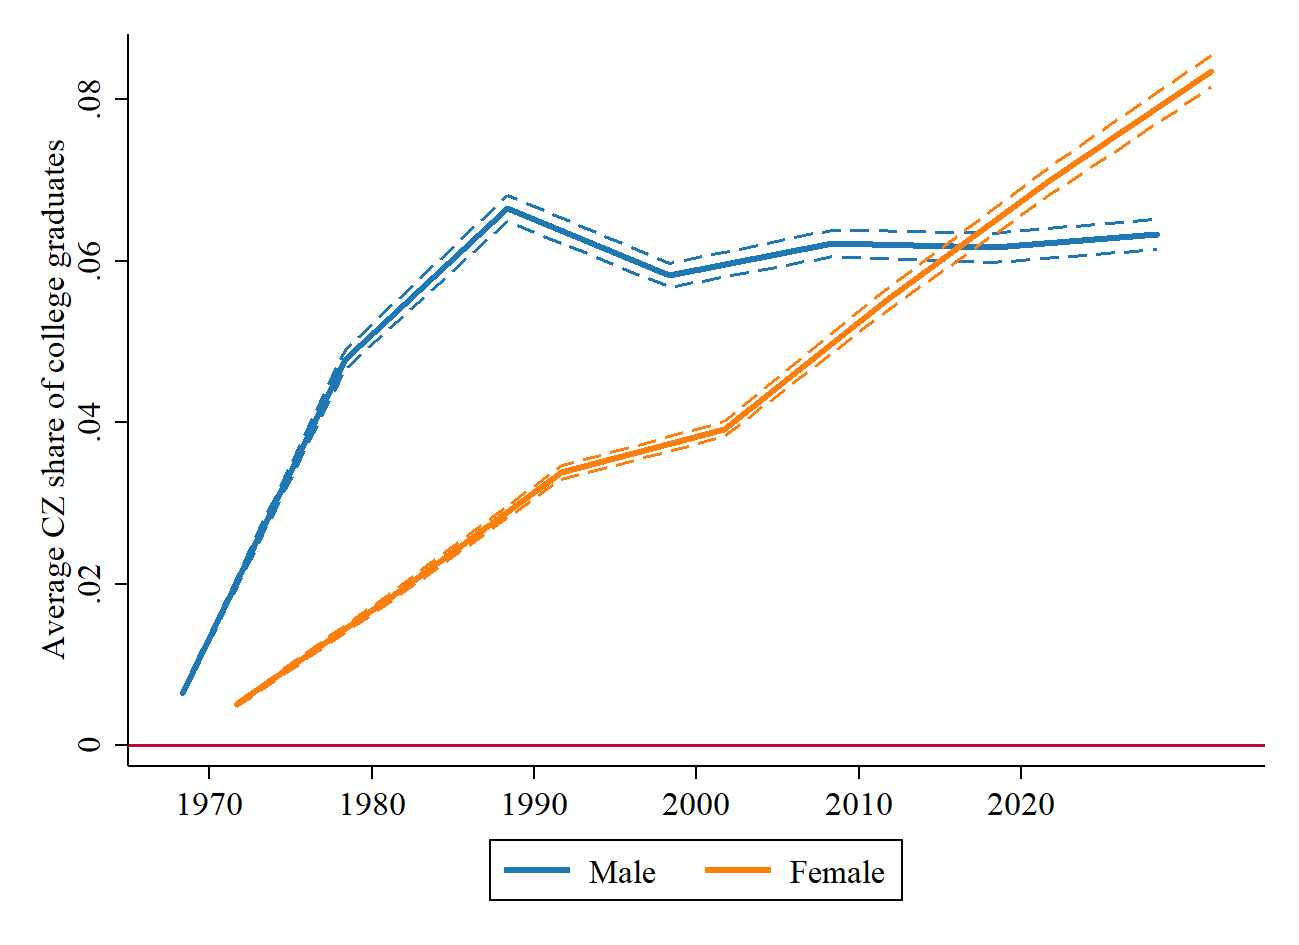
\includegraphics[width=.5\textwidth]{../2_analysis/output/figures/education_share_average}} \subfloat[College share-density gradient]{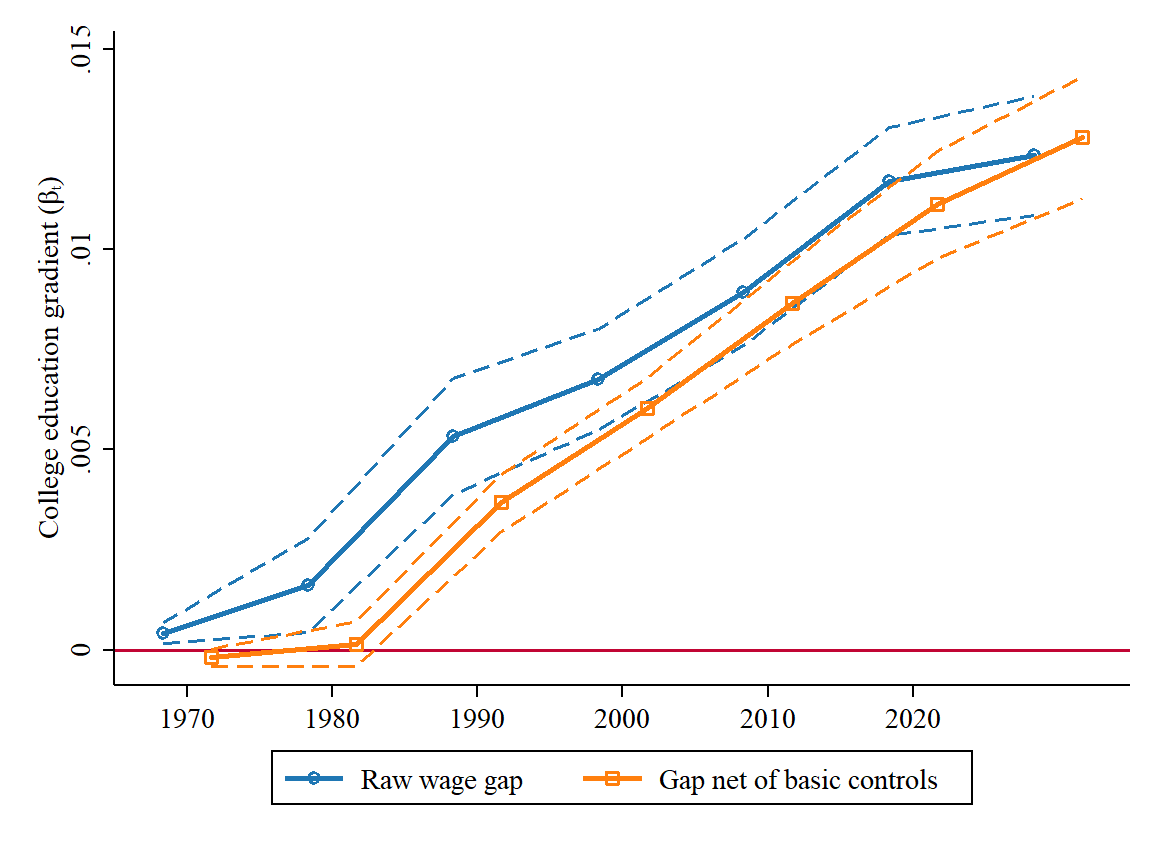
\includegraphics[width=.5\textwidth]{../2_analysis/output/figures/education_share_gradients}} \\ 
\par \begin{minipage}[h]{\textwidth}{\tiny\textbf{Note:} figure restricts to CZ with more than 1 people per km$^2$. Bars show 90\% confidence intervals. Standard errors clustered at the CZ level. Figure generated on 30 Nov 2020 at 11:17:24. Figure generated using the dofile 2\_analysis/code\_files/write\_regression\_coefplots.do.}\end{minipage}
\end{figure}



In panel a of figure \ref{figure:education}, I show estimates of $\beta_{et}$ for the following regression model:
\beqns
w^m_{ret}-w^f_{ret}=\alpha_{et}+\beta_{et}\ln(density)_{rt}
\eeqns
If all the variation is driven by changes in education-specific urban wage premium, then we should expect $\beta_{et}$ to be zero in all years. This is not what the data shows. The gender-gap gradient is positive and mostly constant for college graduates. The decline in the gradient arises for non-college graduates only. Panel b shows that adjusting the gap for age and race does not change this finding (panel b).


Panels c and d show the density premiums by gender. There I plot the density slope in regressions of the form:
\beqns 
	w^g_{ret}=\alpha_{et}^g+\beta_{et}^g\ln(density)_{rt}
\eeqns

\bitem
	\item Women with a bachelor degree benefit \textit{less} from cities than men. Moreover, panel (b) shows that there is no decline in the urban wage premium for college workers. This is consistent with the findings by [autor].
	\item The decline for non college workers happens in both genders. But again, women are less affected by this development $\implies$ \textit{the reversal of fortunes is happening for college without a college education.}
\eitem 

Although education is an endogenous outcome, it is remarkable that the urban wage premium for college graduates is so constant for both genders over the whole period. 
\bitem
	\item Women's labor force participation and educational attainment has increased massively over the years. Moreover, their concentration in urban areas has also increased. If anything, a simple supply-demand framework would have suggested that the gender-gap premium should have decreased.
	\item This begs the question of whether the urban wage premium is smaller for college women. If so, what prevents them from reaping the same benefits as men from cities?
\eitem 

\begin{figure}[!h]
\centering
\caption{The density gradient by education level}
\label{figure:education}
\subfloat[Gender gap gradient]{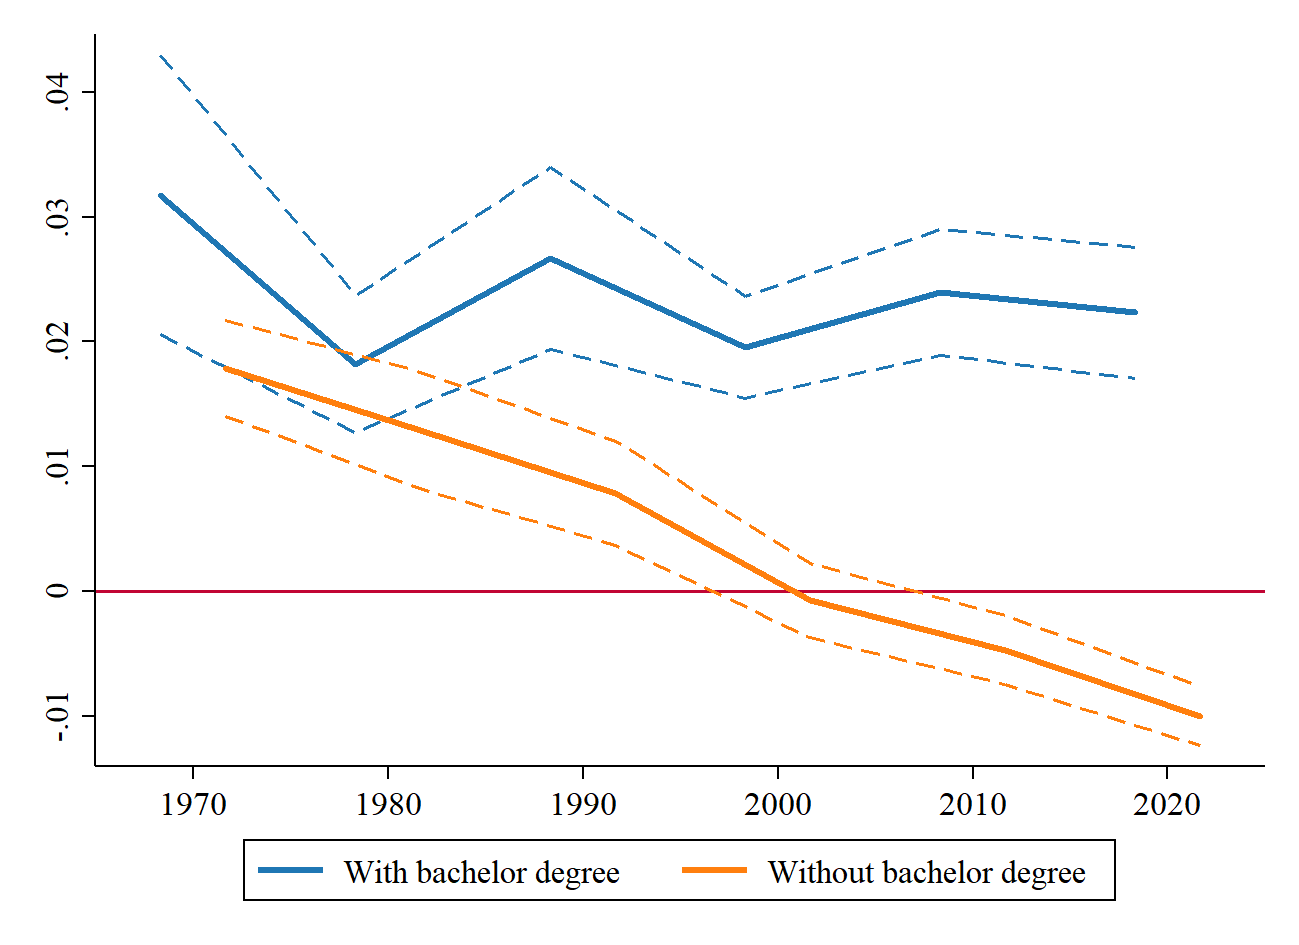
\includegraphics[width=.5\textwidth]{../2_analysis/output/figures/education_gap_full_time}} \subfloat[Gender gap gradient, age and race adjusted]{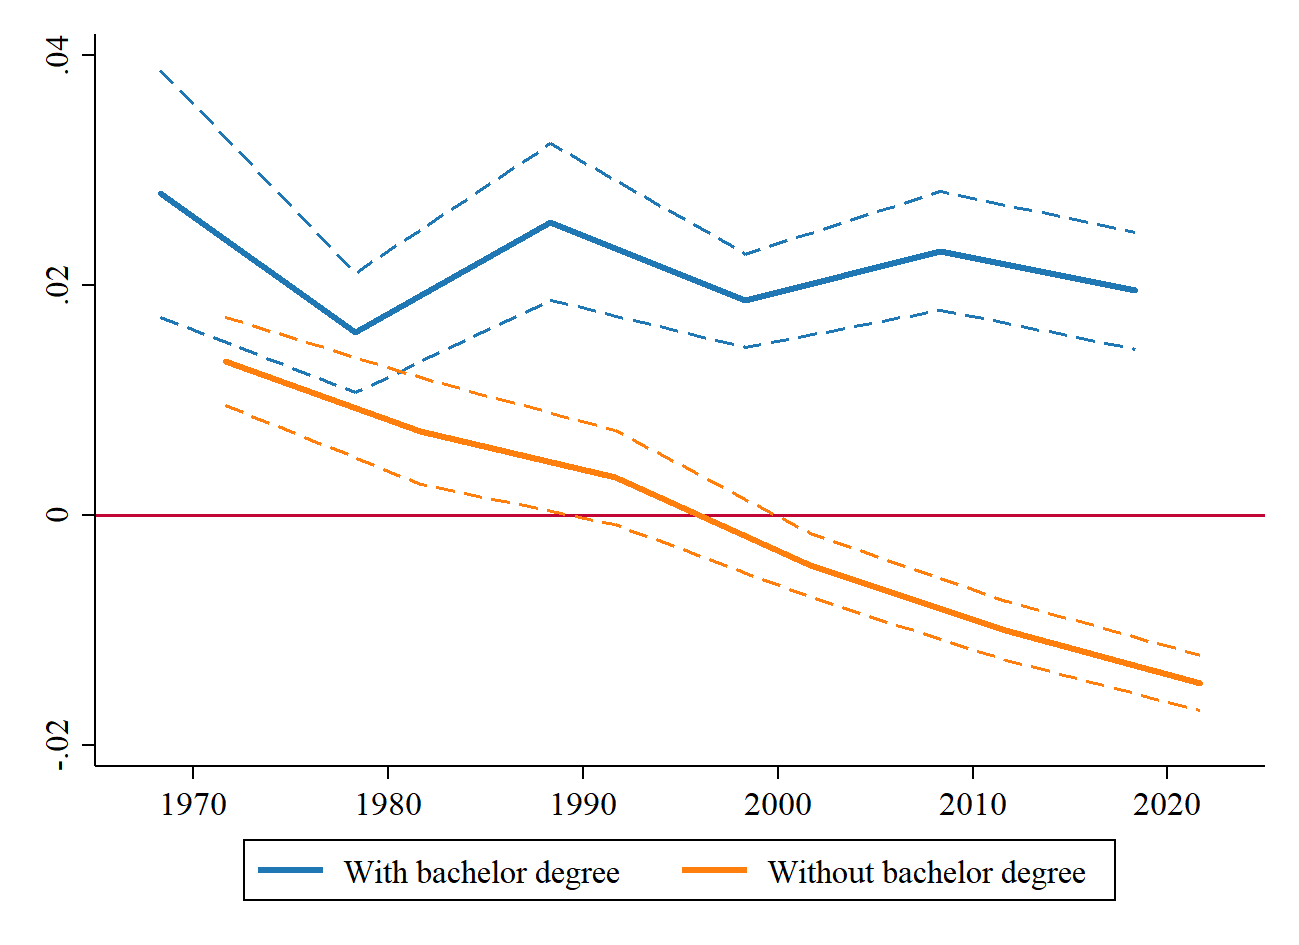
\includegraphics[width=.5\textwidth]{../2_analysis/output/figures/education_gap_bas_full_time}} \\ \subfloat[Urban wage premium (age/race adjusted), with bachelor degree]{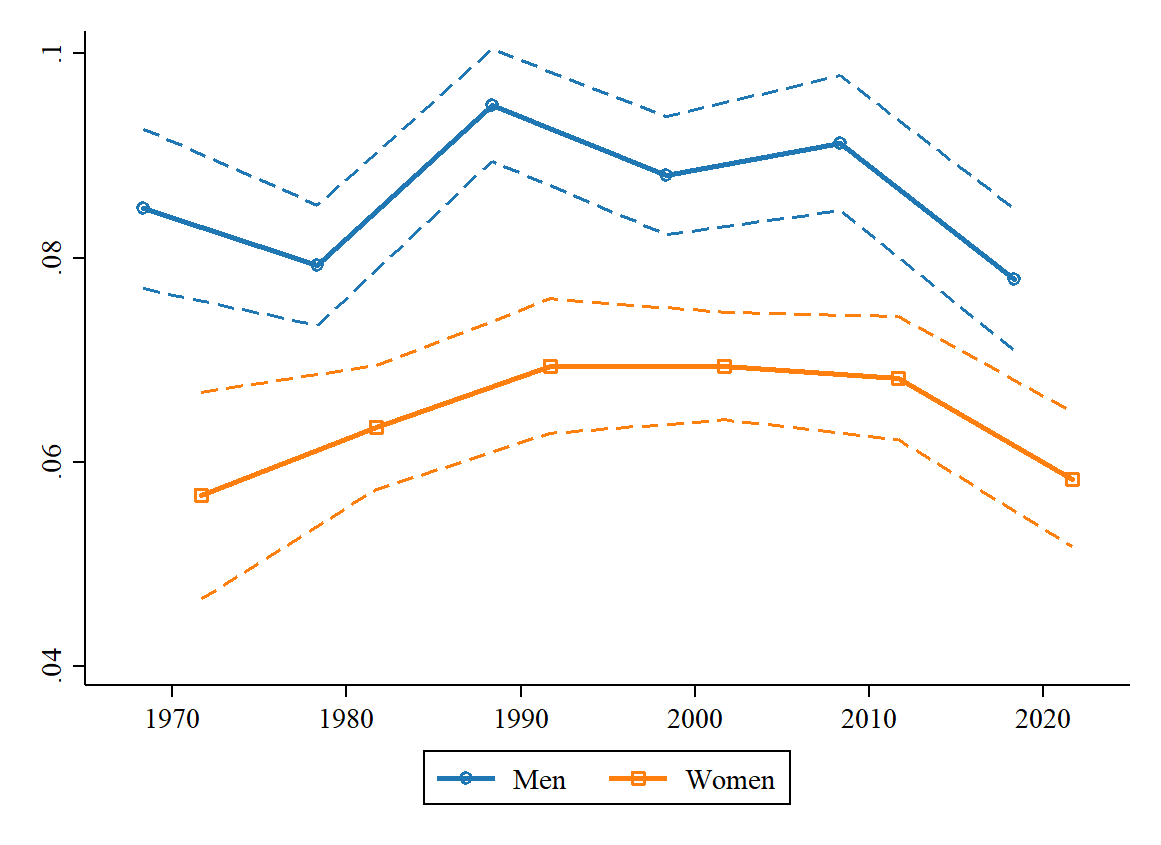
\includegraphics[width=.5\textwidth]{../2_analysis/output/figures/education_high_premium_full_time}} \subfloat[Urban wage premium (age/race adjusted), without bachelor degree]{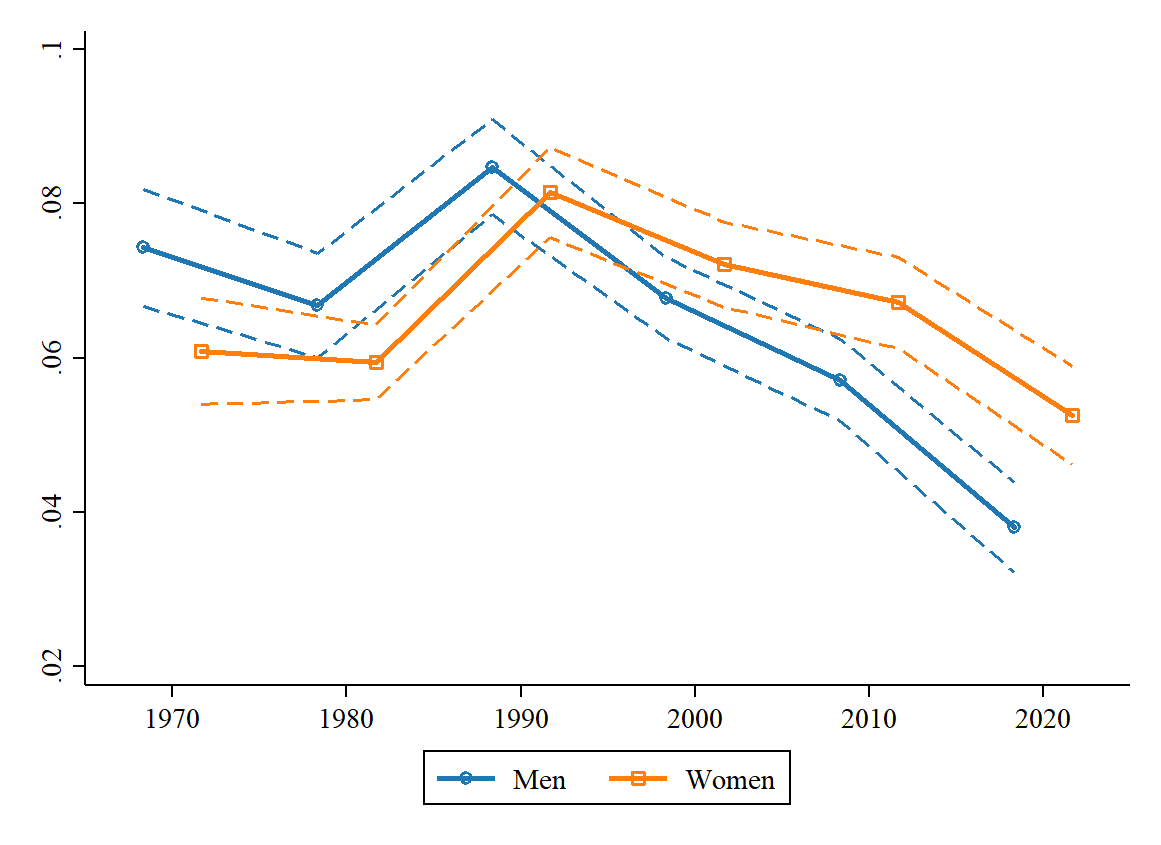
\includegraphics[width=.5\textwidth]{../2_analysis/output/figures/education_low_premium_full_time}} \\ 
\par \begin{minipage}[h]{\textwidth}{\tiny\textbf{Note:} figure restricts to CZ with more than 1 people per km$^2$. Dashed lines represent 90\% confidence intervals. Figure generated on 23 Nov 2020 at 11:41:43. Figure generated using the dofile 2\_analysis/code\_files/write\_regression\_coefplots.do.}\end{minipage}
\end{figure}


\subsection{1970-1990}

Figure \ref{fig:controls} suggests that industry of employment accounts for both the (i) cross-sectional gender-gap gradient, and (ii) its decline during 1990-2020. Here I zoom in on the relationship between industrial structure, population density, and employment shares across genders.

\subsubsection{What are the high pay industries?}

Figure \ref{fig:which_pay} shows two main facts:
\bitem
	\item High pay industries are primarily manufacturing in 1970-2020.
	\item Over time, high-pay industries become more service-intensive.	
\eitem 

\begin{figure}[!h]
\centering
\caption{Industries and relative pay}
\label{fig:which_pay}
\subfloat[Relative pay in 2020 vs 1970]{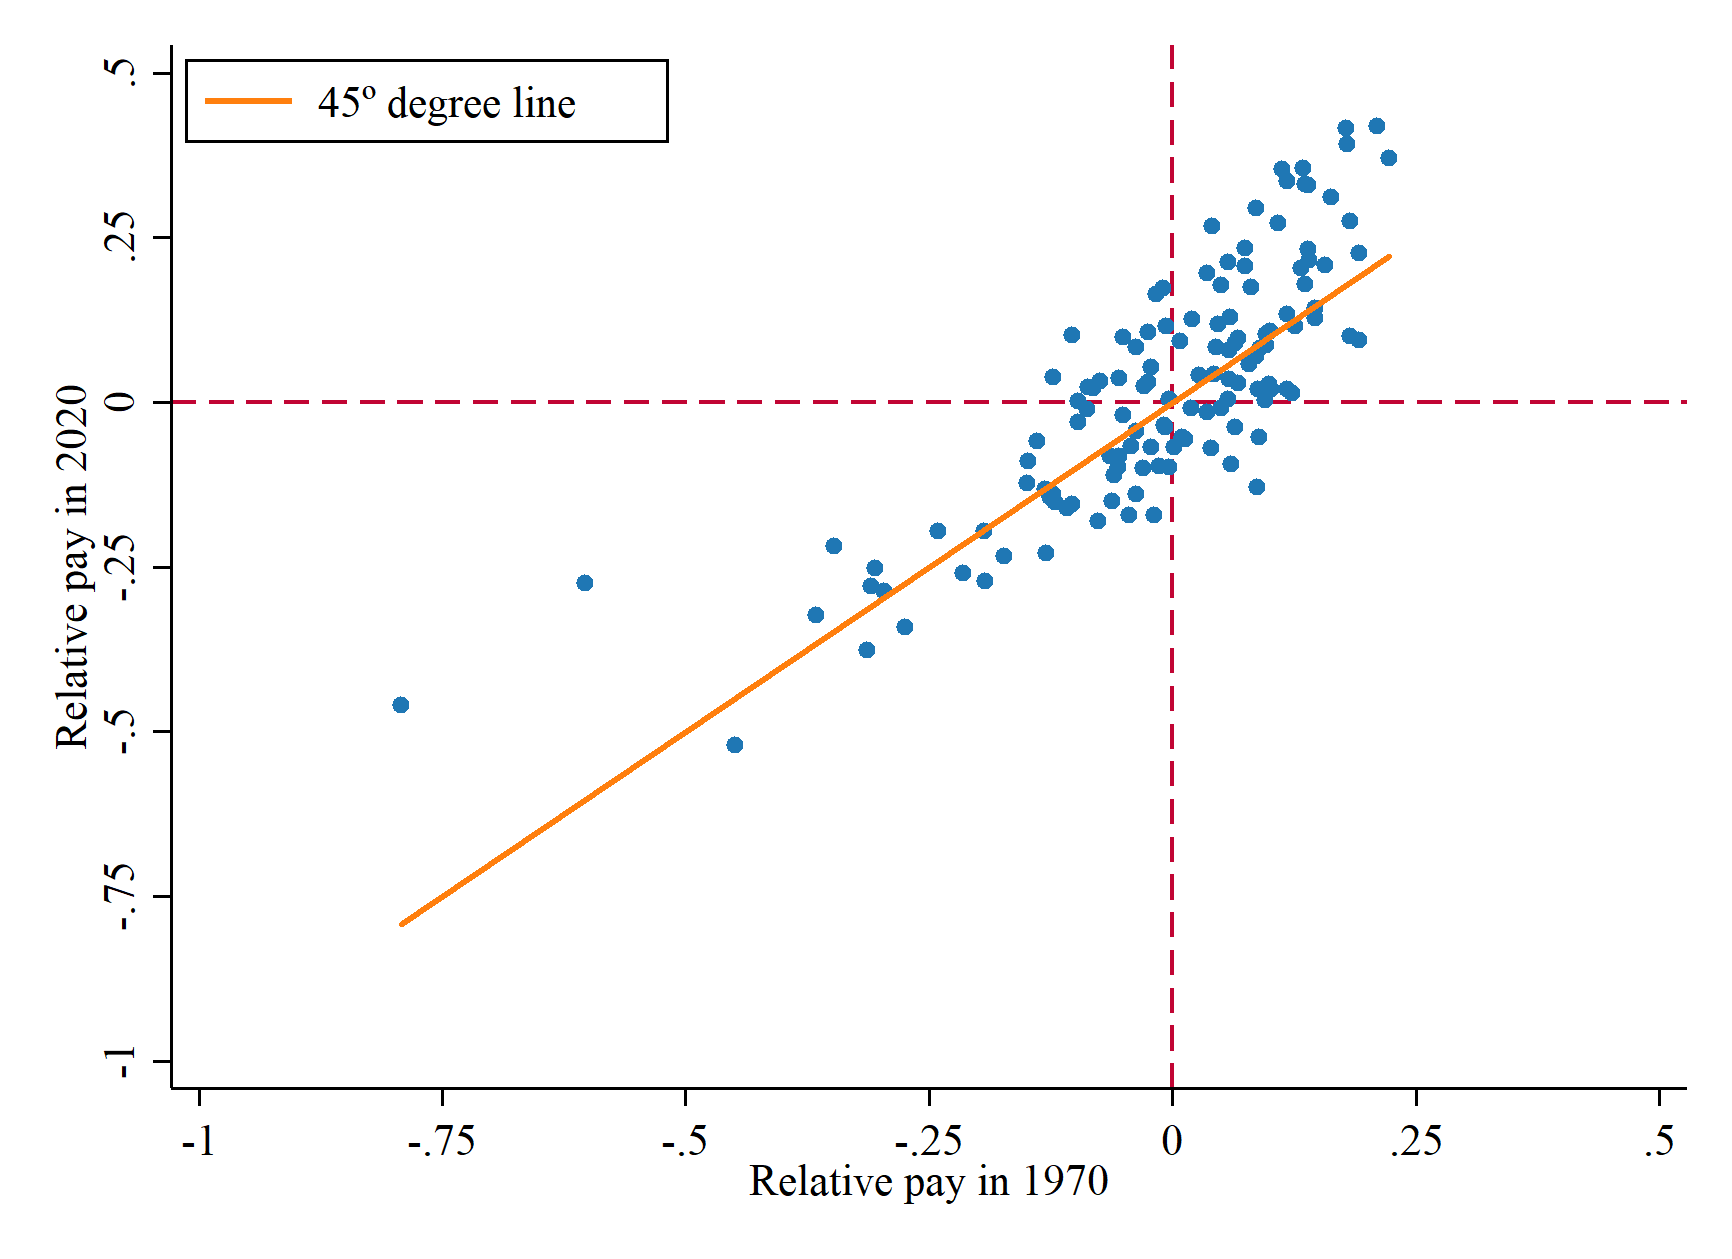
\includegraphics[width=.5\textwidth]{../2_analysis/output/figures/ranking_persistence}} \subfloat[High-pay industries by industry-group]{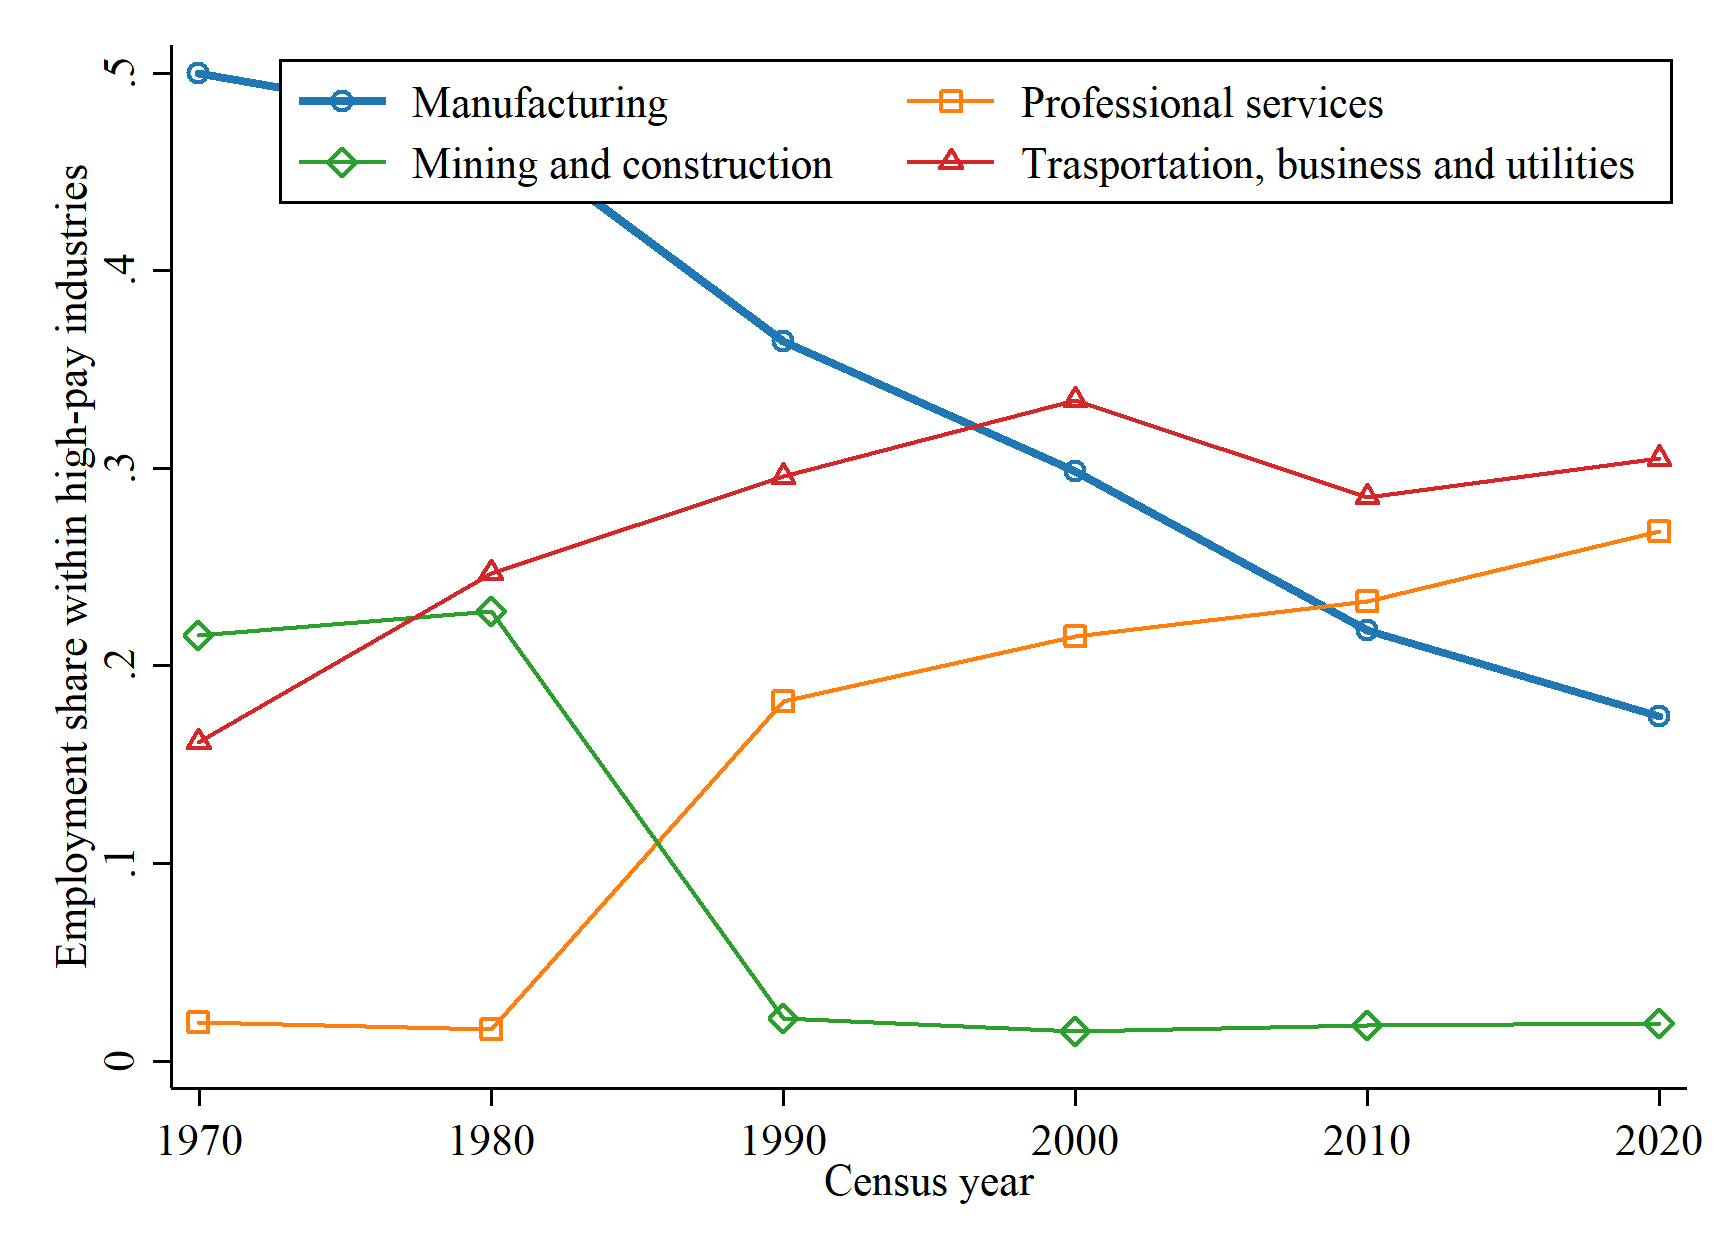
\includegraphics[width=.5\textwidth]{../2_analysis/output/figures/high_pay_by_type}} \\ 
\par \begin{minipage}[h]{\textwidth}{\tiny\textbf{Note:} figure restricts to CZ with more than 1 people per km$^2$. Figure generated on 30 Nov 2020 at 23:01:52.}\end{minipage}
\end{figure}


\subsubsection{Women are less likely to be employed in high pay industries}

I include 147 industry classifications. 

First I show that there are differences across gender in the likelihood of being employed in a high pay industry. For this I run the regression:

\beqns
	s_{t}^g=\alpha_t^g+\beta^g_t\lambda_{jt}
\eeqns
where $s_{t}^g$ indicates the nation-wide employment share of gender $g$ in industry $j$, and $\lambda_jt$ represents the industry fixed effect obtained in the first stage regressions.

\begin{figure}[!h]
\centering
\caption{Industry employment share by gender}
\label{figure:ind_gender_shares}
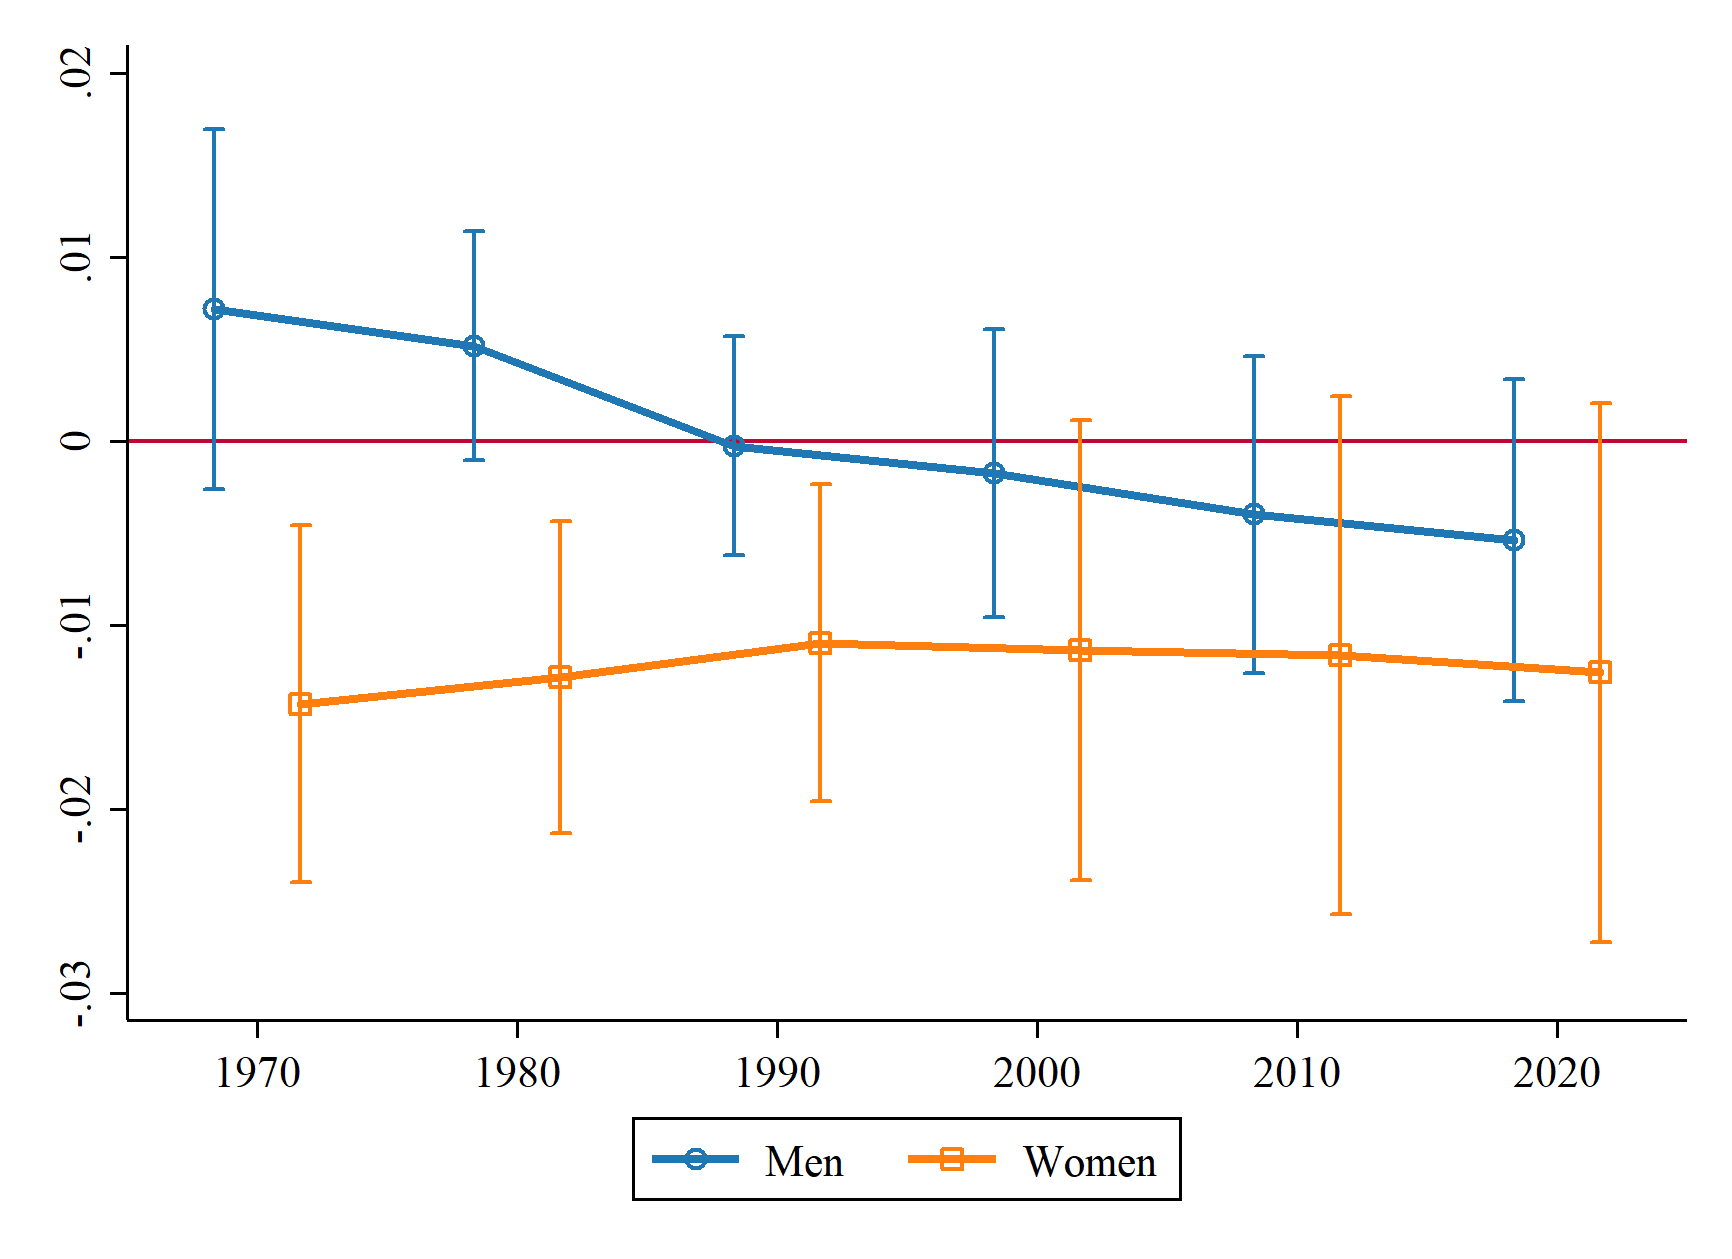
\includegraphics[width=1\textwidth]{../2_analysis/output/figures/gender_ind_empshares}
\par \begin{minipage}[h]{\textwidth}{\tiny\textbf{Note:} figure restricts to CZ with more than 1 people per km$^2$. Bars show 90\% confidence intervals. Standard errors clustered at the CZ level. Figure generated on 30 Nov 2020 at 23:01:43.}\end{minipage}
\end{figure}


\begin{figure}[!h]
\centering
\caption{Industry employment distribution by gender}
\label{fig:gender_distribution}
\subfloat[Ranking fixed in 1970]{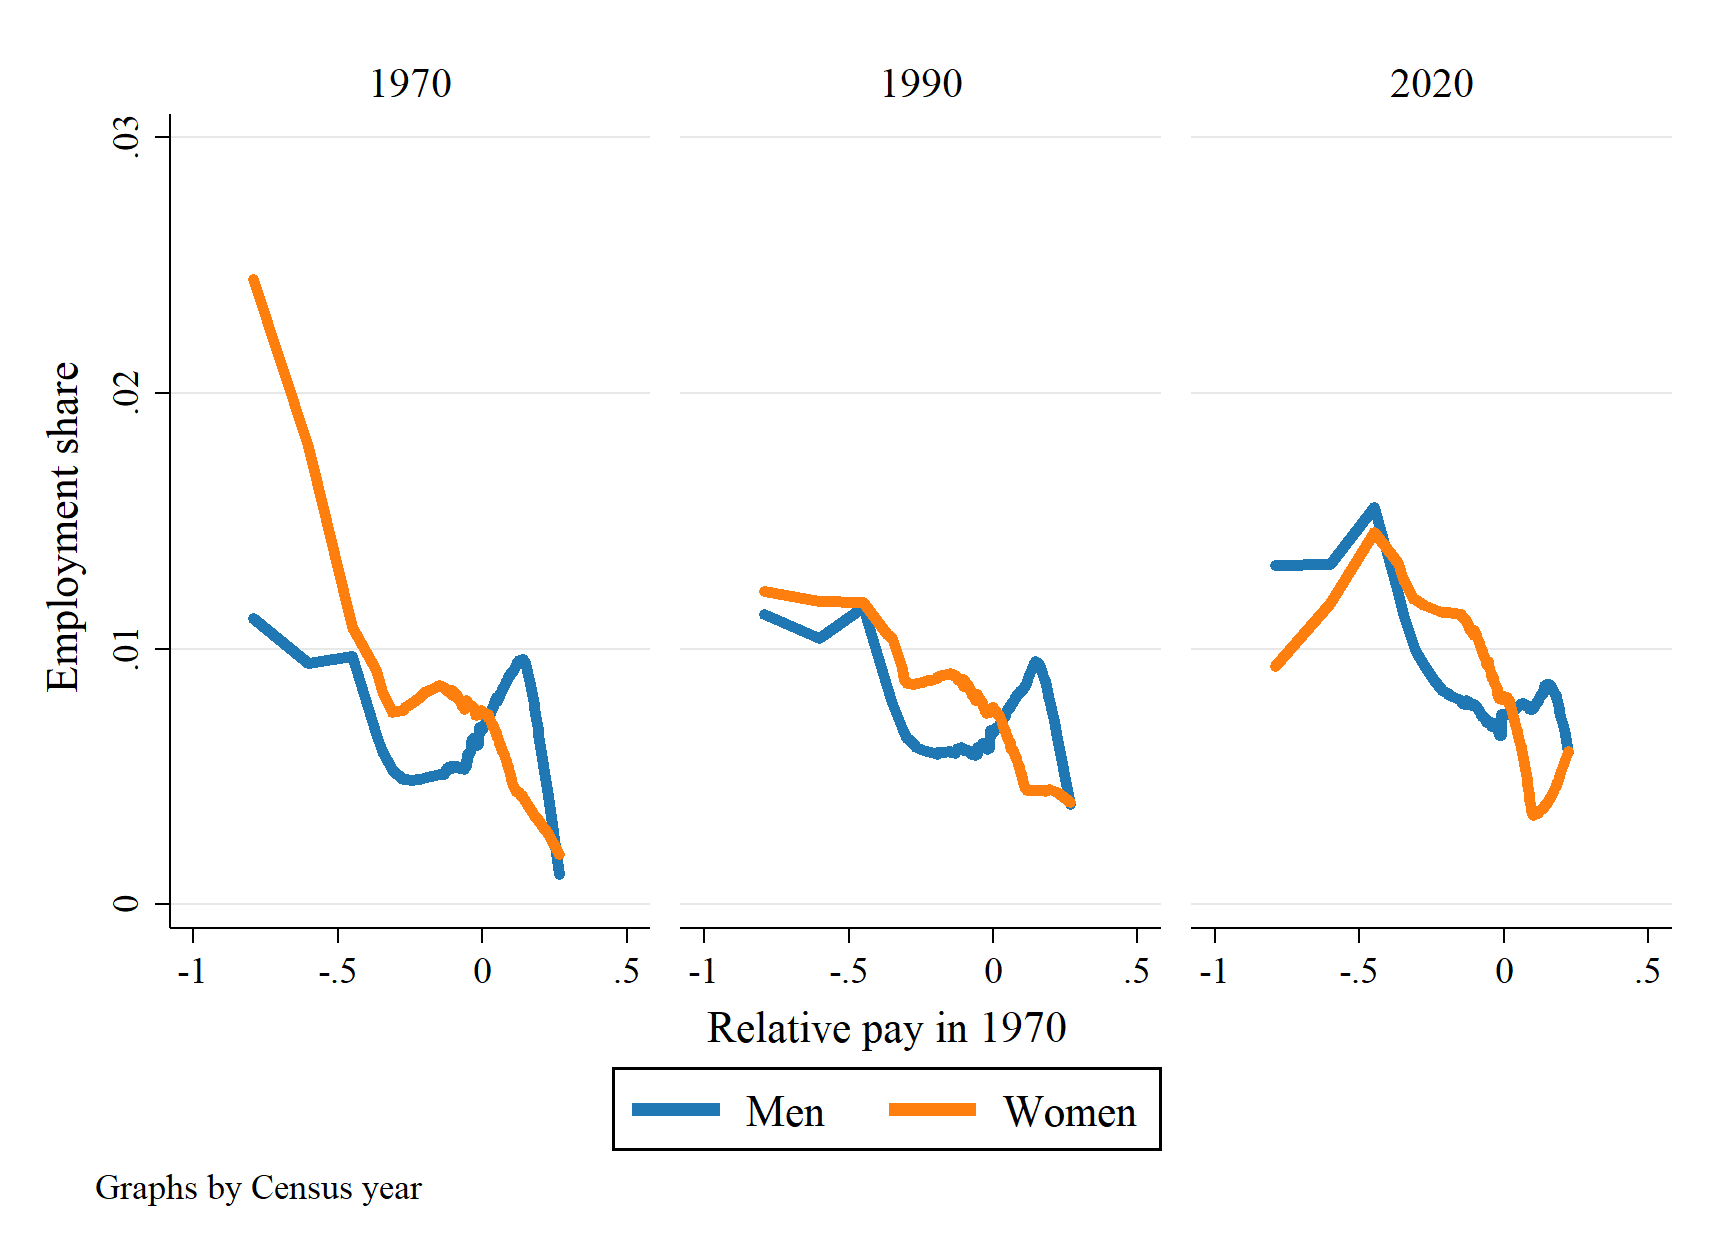
\includegraphics[width=.5\textwidth]{../2_analysis/output/figures/gender_empshare_distribution}} \subfloat[Varying the ranking]{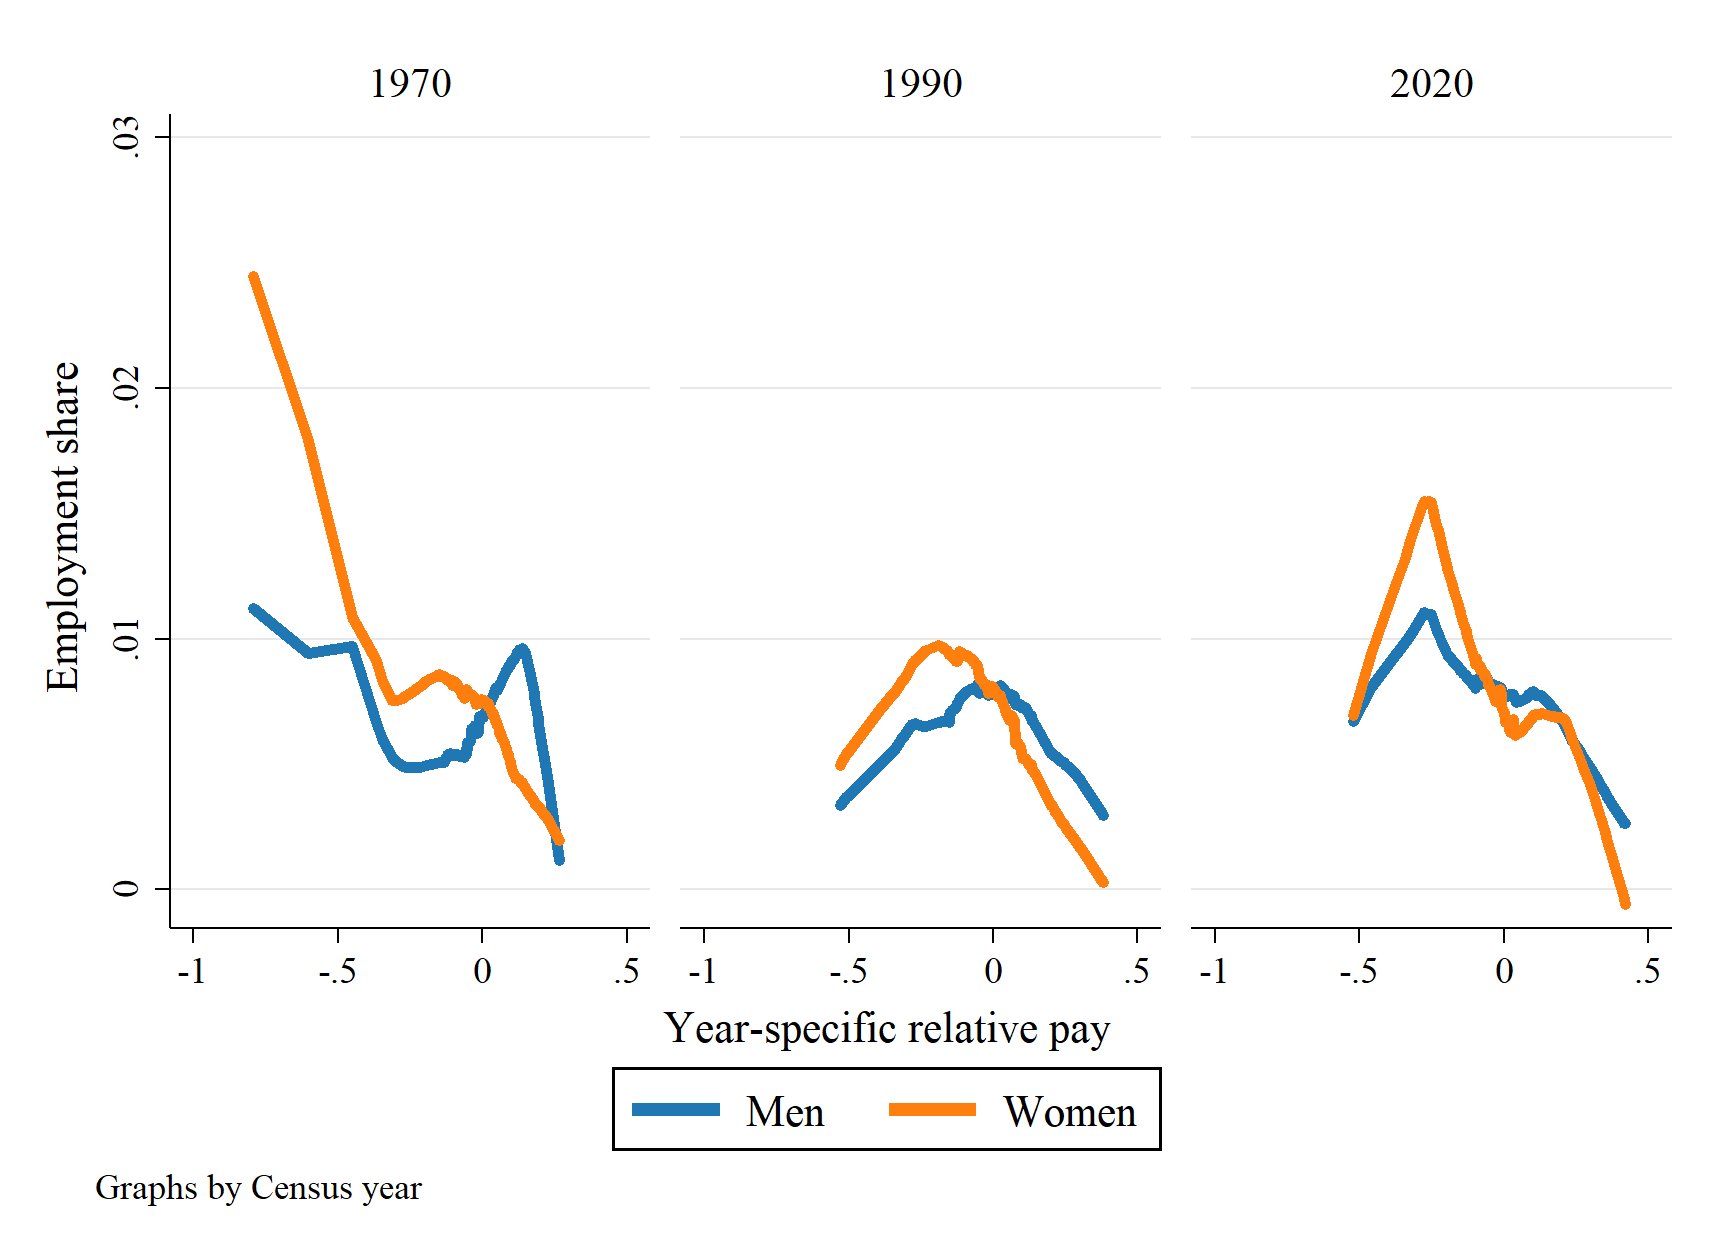
\includegraphics[width=.5\textwidth]{../2_analysis/output/figures/gender_empshare_distribution_year_ranking}} \\ 
\par \begin{minipage}[h]{\textwidth}{\tiny\textbf{Note:} figure restricts to CZ with more than 1 people per km$^2$. Figure generated on 30 Nov 2020 at 23:01:48.}\end{minipage}
\end{figure}


Figure \ref{figure:ind_gender_shares} shows the estimated $\beta^g$ for both genders.

Two features that stand out:
\bitem
	\item On average women are less likely to be employed in the high wage industries. That said, estimates become much noisier from 1990 onward.
	\item There's a slight downward trend in men's likelihood of being employed in high-wage industries.
\eitem
Panel a of figure \ref{fig:gender_distribution} gives a more detailed description of the employment distributions by gender. Women in 1970 are primarily concentrated in low-pay industries, but over 1970 to 1990, they gained access to industries with better pay. 


Men's evolution is also interesting. A comparison between panels (a) and (b) in \ref{fig:gender_distribution} reveals two facts:
\benu
	\item In 1970, men are highly concentrated in industries at the top of the pay distribution. Panel (a) also shows that there is persistence in this employment distribution. They continue to concentrated in industries that were high pay in 1970, even in 2020.
	\item However, panel (b) that the industry ranking has changed, so that from 1990 onward, men are not as concentrated in high-pay industries as panel (b) suggests $\implies$ men's jobs are in relative decline \textit{at the national level} 
\eenu
In parallel, men stat the period with a high concentration in high-pay industries, but this concentration diffuses over time.

 Panel b also shows that even though men are still disproportionately concentrated on industries that were highly-paid in 1970, they are no longer high pay by the end of the period.

All in all, this exercise suggests that women's employment distribution is becoming more like men's. But this happens in part by men being less likely to be employed in high-wage industries.

\subsubsection{High pay industries are larger in denser cities}


Figure \ref{fig:ind_cities} studies the relationship between high-pay industries and population density. To construct this figure, first I define an industry as being high-pay, it is in the top tercile of the national relative-pay rank. Rankings are computed separately for each year. Next I compute the CZ-level employment shares in high-pay industries.
\bitem
	\item Panel (a) shows that dense cities are highly specialized in high-pay industries. However, this specialization decreases over time.
	\item Panel (b) shows a similar pattern as the scatterplots. There I plot the slope coefficient in the regression:
	\beqns
		s_{rt}^{high pay}=\alpha_t+\beta_{}\ln(density)_{rt}
	\eeqns
	the ``fixed ranking'' line computes the employment shares when the industry pay rank is fixed to 1970 values. The ``variable ranking'' allows the ranking to change over time. Either way, the message is the same: dense cities were highly specialized in high-pay-industries, but this specialization reduces over time.
\eitem


Ten industries disappear over the  sample period. Check what is happening to them

\begin{figure}[!h]
\centering
\caption{High wage industries and population density}
\label{fig:ind_cities}
\subfloat[Scatterplots by year]{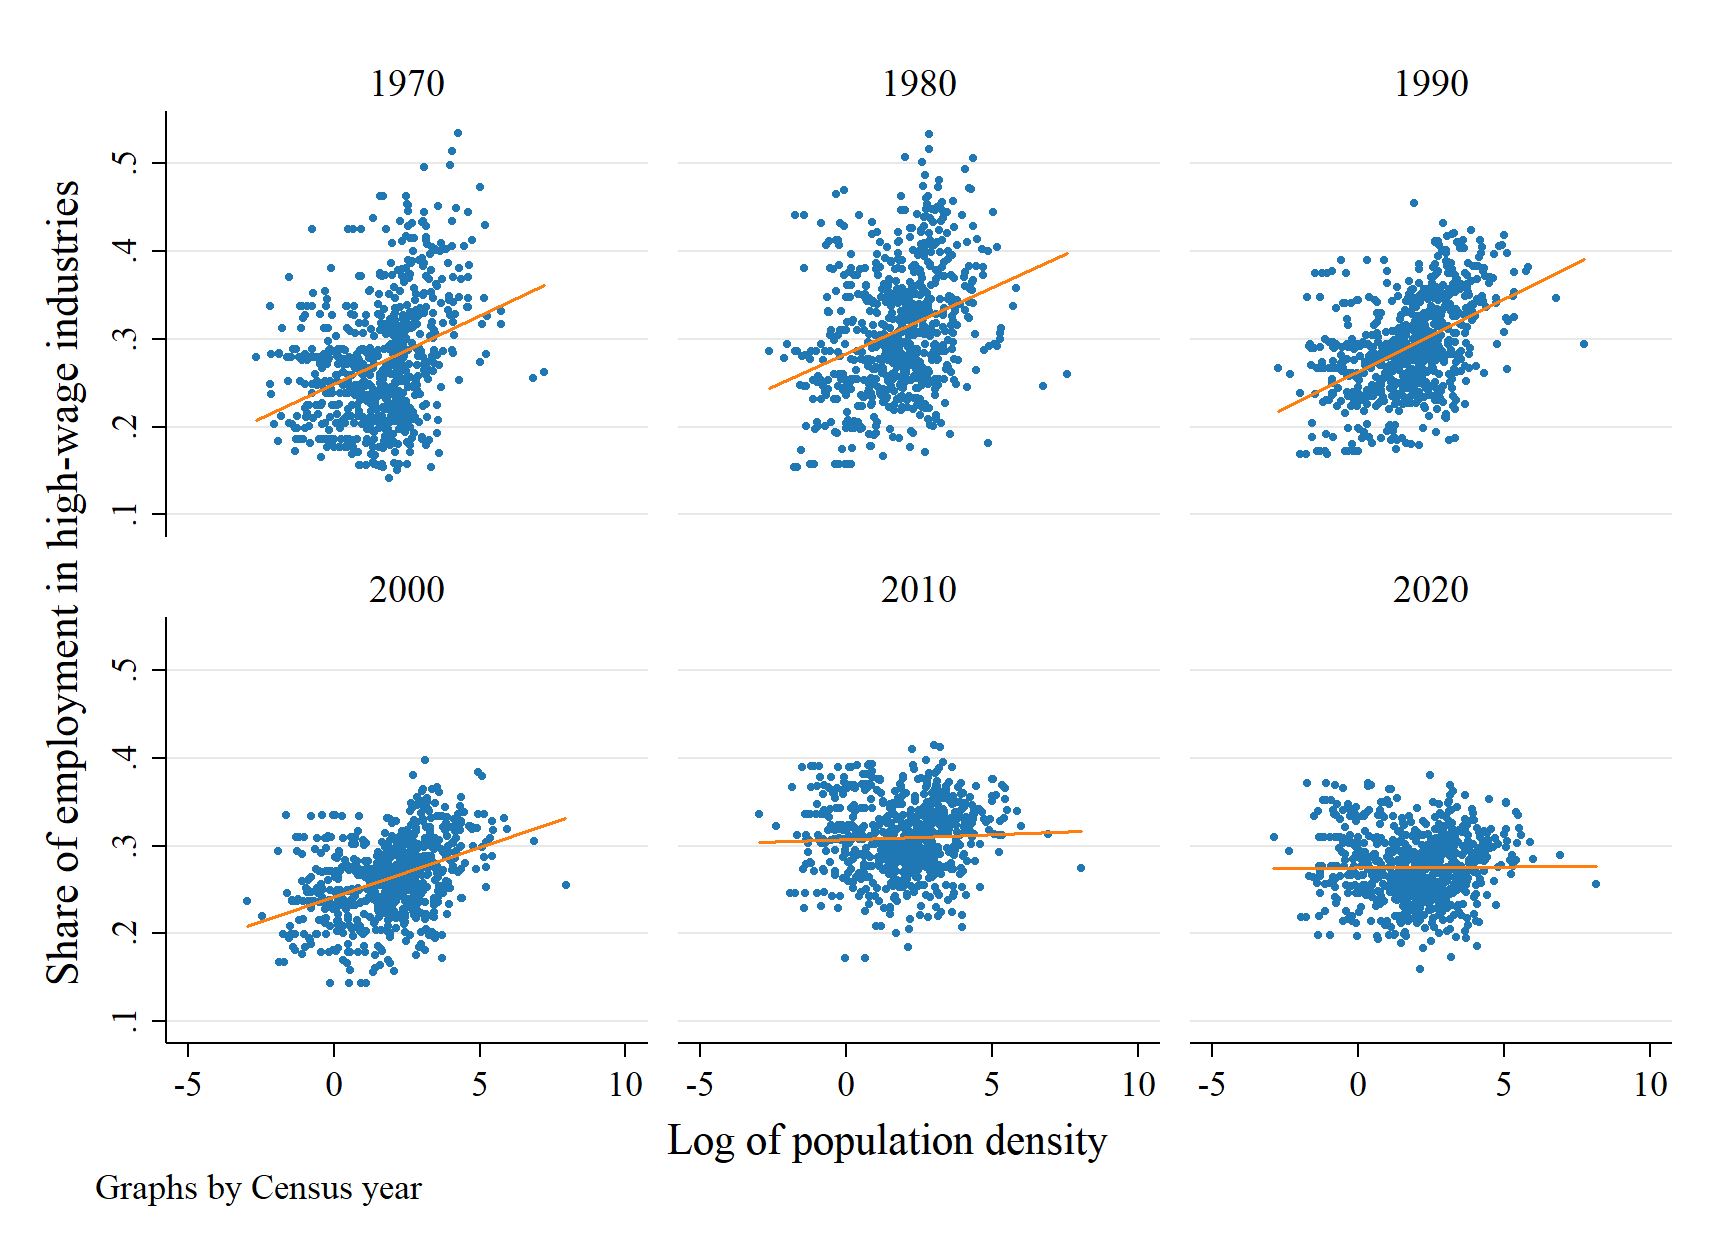
\includegraphics[width=.5\textwidth]{../2_analysis/output/figures/high_wage_ind_city_scatter}} \subfloat[Density gradient]{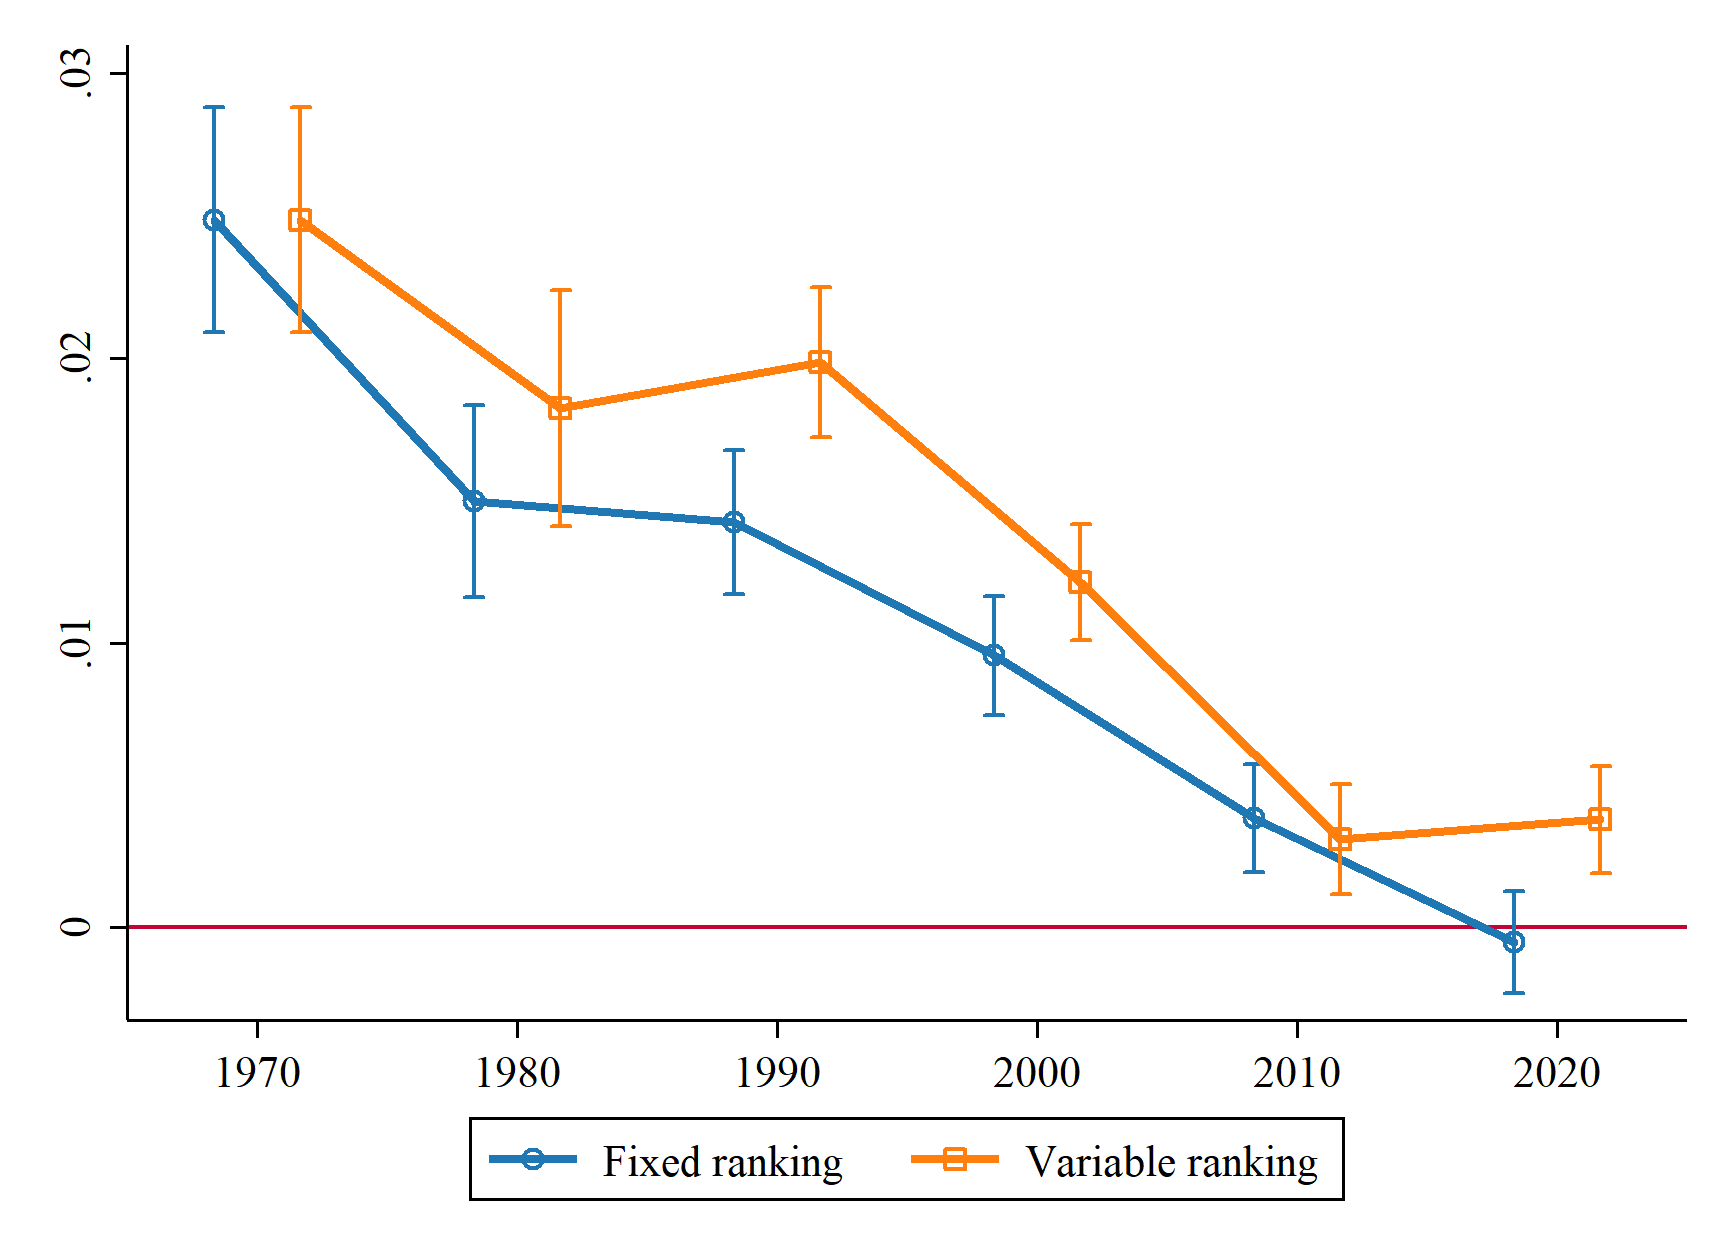
\includegraphics[width=.5\textwidth]{../2_analysis/output/figures/high_wage_ind_city_coefplot}} \\ 
\par \begin{minipage}[h]{\textwidth}{\tiny\textbf{Note:} figure restricts to CZ with more than 1 people per km$^2$. Figure generated on 30 Nov 2020 at 23:01:57.}\end{minipage}
\end{figure}




\subsubsection{Can the industrial composition alone account for the gender-gap gradient?}
Yes, at least for the 1970-1990. To test this let's decompose the change in wages into a part that reflects only changes in the industrial employment distribution, and a second component that reflects only changes in average wages. Note that,
\beqns
w_{rt}^g-w_{r1970}^g=\sum_j(s_{rjt}^g-s_{rj1970}^g)w^g_{rjt}+\sum_js^g_{rj1970}(w_{rjt}^g-w_{rj1970}^g)
\eeqns
\bitem
	\item $\sum_j(s_{rjt}^g-s_{rj1970}^g)w^g_{rjt}$: captures only changes in the employment distribution over time.
	\item $\sum_js^g_{rj1970}(w_{rjt}^g-w_{rj1970}^g)$ captures only changes in the industrial average wages.
\eitem
Then if we consider the following two regressions:
\beqns
	w_{rt}&=&\alpha_{t} + \beta_t\ln(density)_{rt}\\
\sum_js^g_{rj1970}w_{rjt}^g&=&\bar{\beta}_{t} + \bar{\beta}_t\ln(density)_{rt}
\eeqns
Then following the above decomposition we can readily interpret the density coefficients as follows:
\bitem
	\item $\beta_t-\bar{\beta}_t$: change in the urban wage premium explained by changes in the industrial employment distribution.
	\item $\bar{\beta}_t-\beta_{1970}$: change in the urban wage premium that is explained by the evolution of industrial average wages.
\eitem 

\begin{figure}[!h]
\centering
\caption{Coefficient on population density $ \beta_t $}
\label{figure:fixed_shares}
\subfloat[Fixed employment shares]{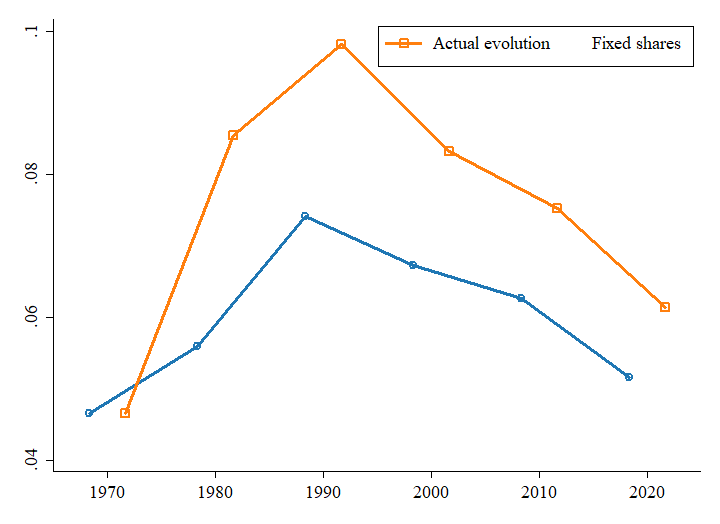
\includegraphics[width=.5\textwidth]{../2_analysis/output/figures/fixed_shares_exercise}} \subfloat[Fixed employment shares vs fixed wages]{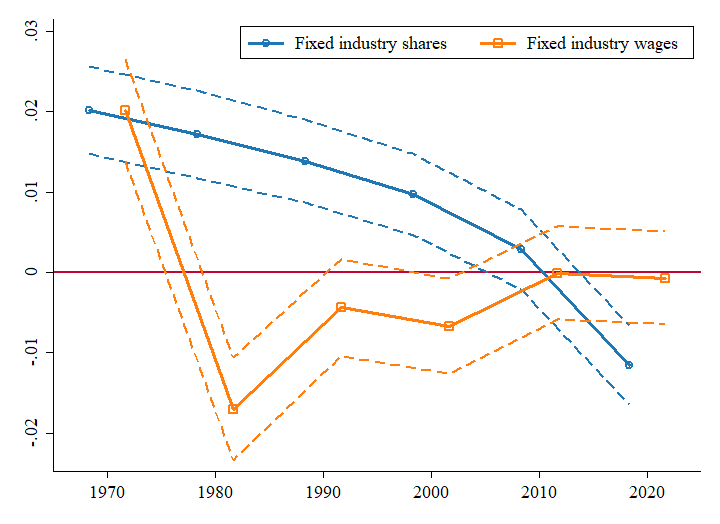
\includegraphics[width=.5\textwidth]{../2_analysis/output/figures/fixed_shares_exercise_wage}} \\ 
\par \begin{minipage}[h]{\textwidth}{\tiny\textbf{Note:} figure restricts to CZ with more than people per km$^2$. Bars show 90\% confidence intervals. Standard errors clustered at the CZ level. Figure generated on  2 Dec 2020 at 13:48:43.}\end{minipage}
\end{figure}


















Taking the model presented in the previous 
Following the wage model presented in previous sections, the industry fixed effects account for the density gradient as long as there are differences by gender in the employment distributions by gender. As a quick check, consider the regression:
\beqns
gap_{rt}=\alpha_t+\beta_{t}\ln(density)_{rt}+\chi_t(s_{rt}^{highpay,m}-s_{rt}^{highpay,f})+\delta_ts_{rt}^{highpay,m}sh
\eeqns
where $s_{rt}^{highpay,g}$ is the employment share in high-pay industries for gender $g$. Panels (a) and (b) of figure \ref{fig:high_wage_gradients} show the coefficient on density in the above regression. Two facts stand out:
\benu
\item Most of the cross-sectional correlation between density and the gender gap during the period 1970-1990 is accounted for the share of employment in high-pay industries.
\item Adding these additional regressors also accounts for \textit{change in the gradient over this period}. 
\eenu

\begin{figure}[!h]
\centering
\caption{High wage industries by gender}
\label{fig:high_wage_gradients}
\subfloat[Net-of race/age gender gap and high-wage industry share]{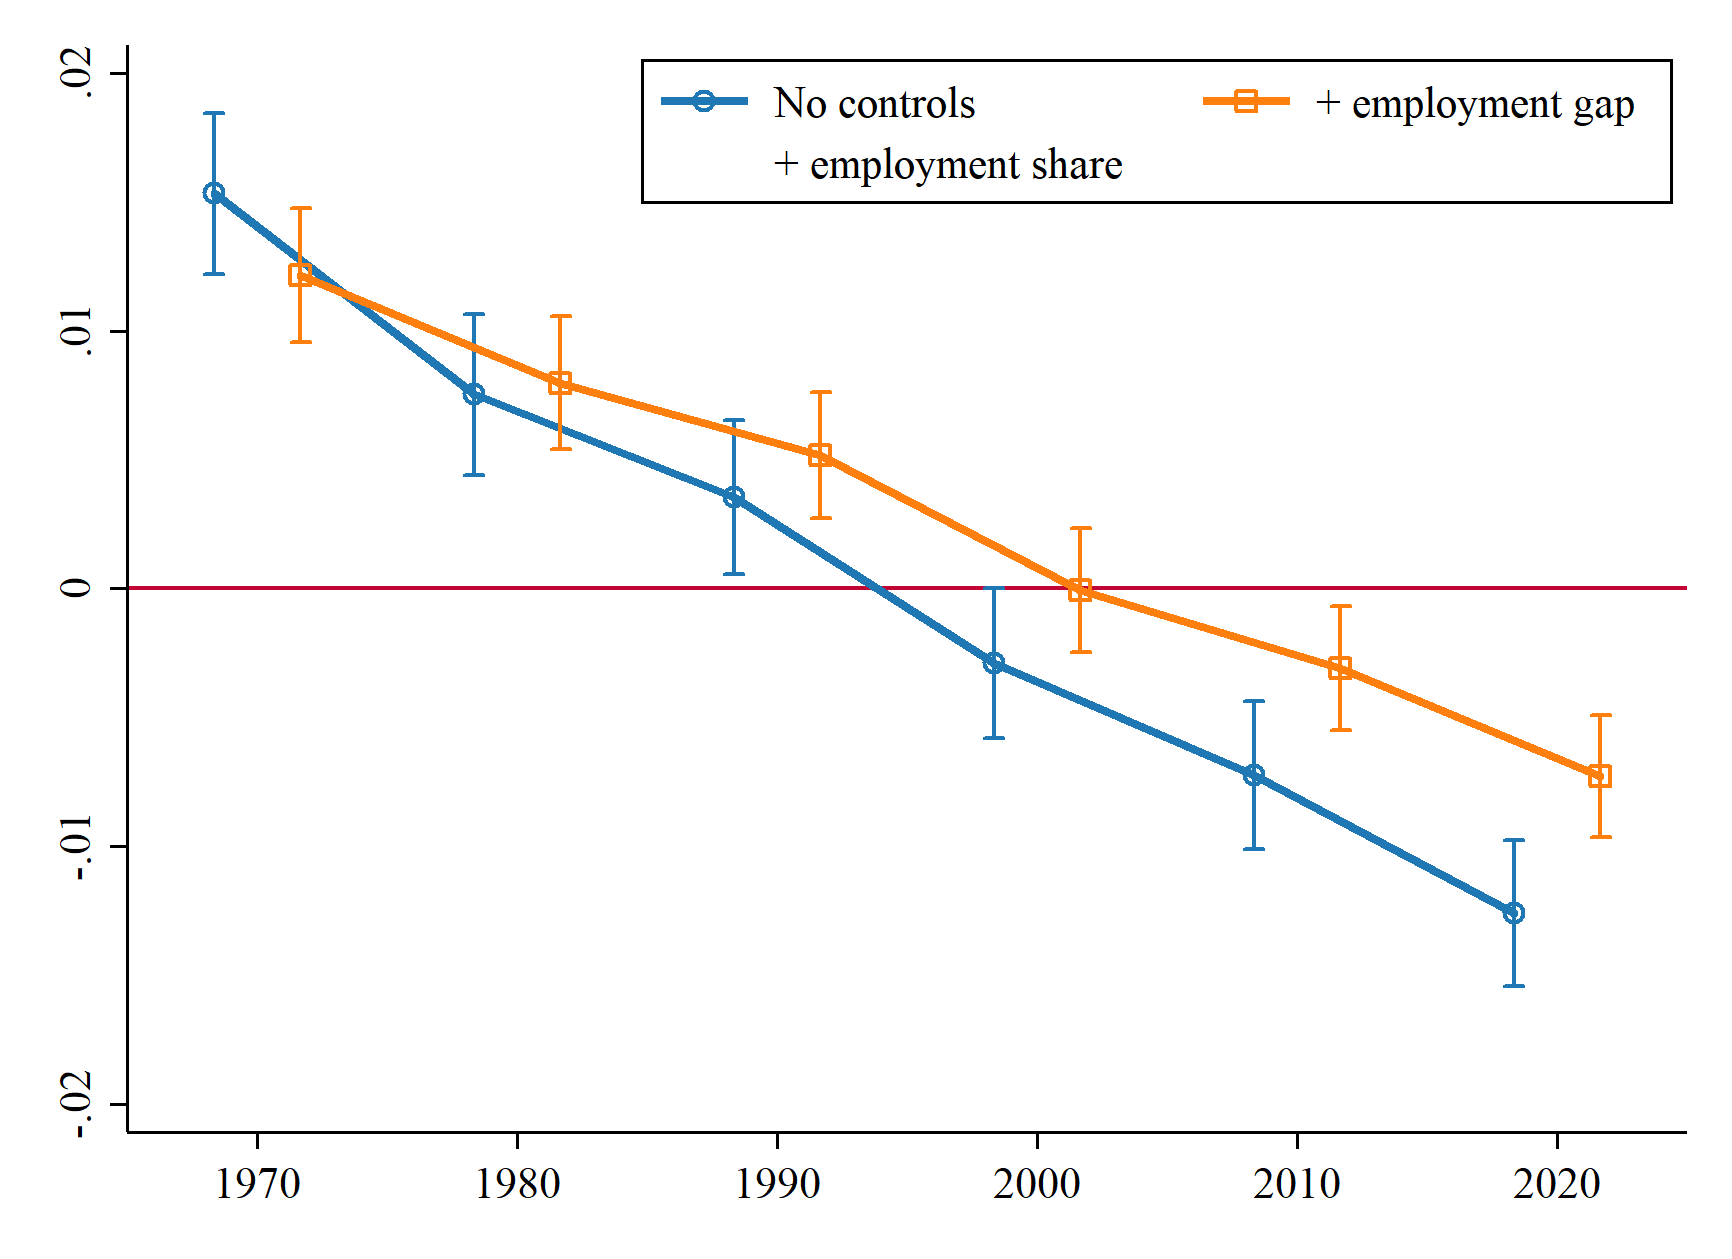
\includegraphics[width=.5\textwidth]{../2_analysis/output/figures/gender_bas_gap_gradient_high_share}} \subfloat[Net-of-education gap and high-wage industry share]{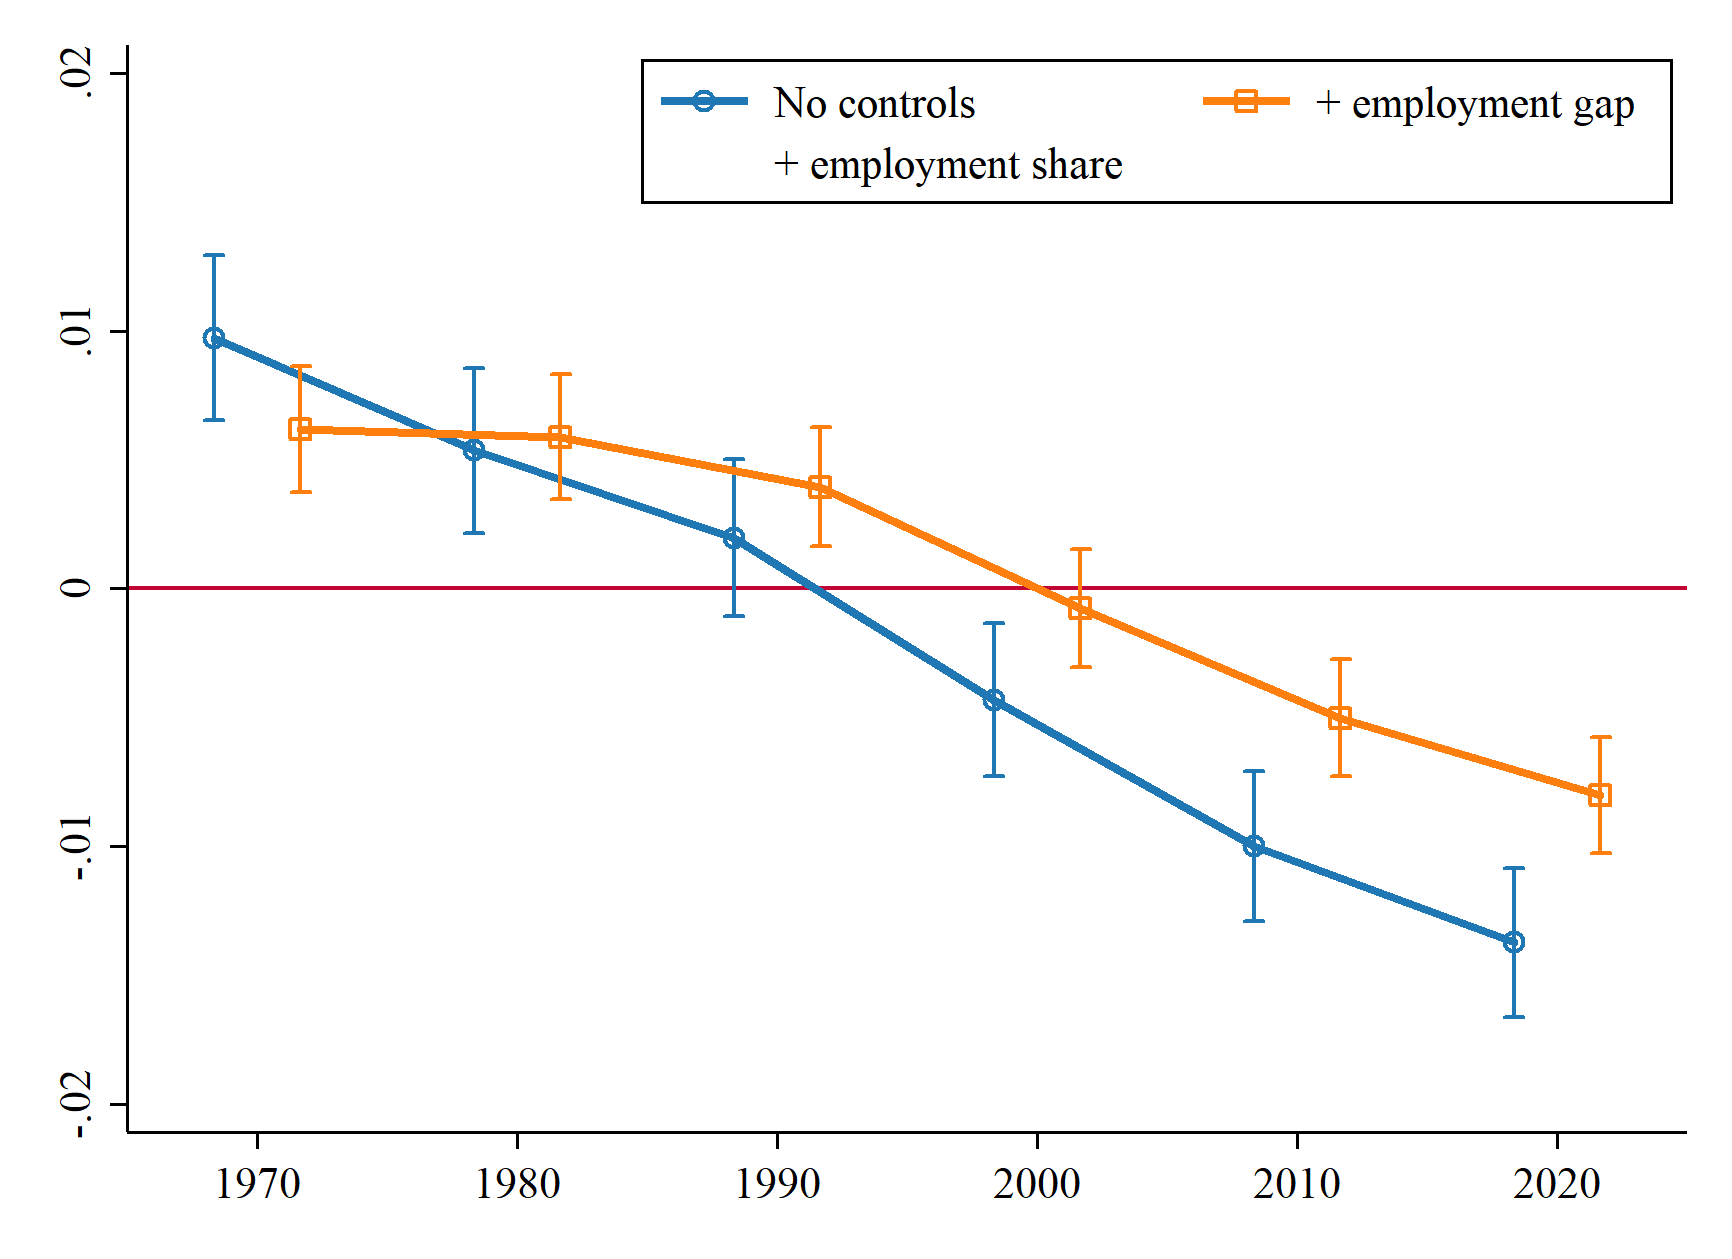
\includegraphics[width=.5\textwidth]{../2_analysis/output/figures/gender_hum_gap_gradient_high_share}} \\ \subfloat[Men's high-wage industry employment, men]{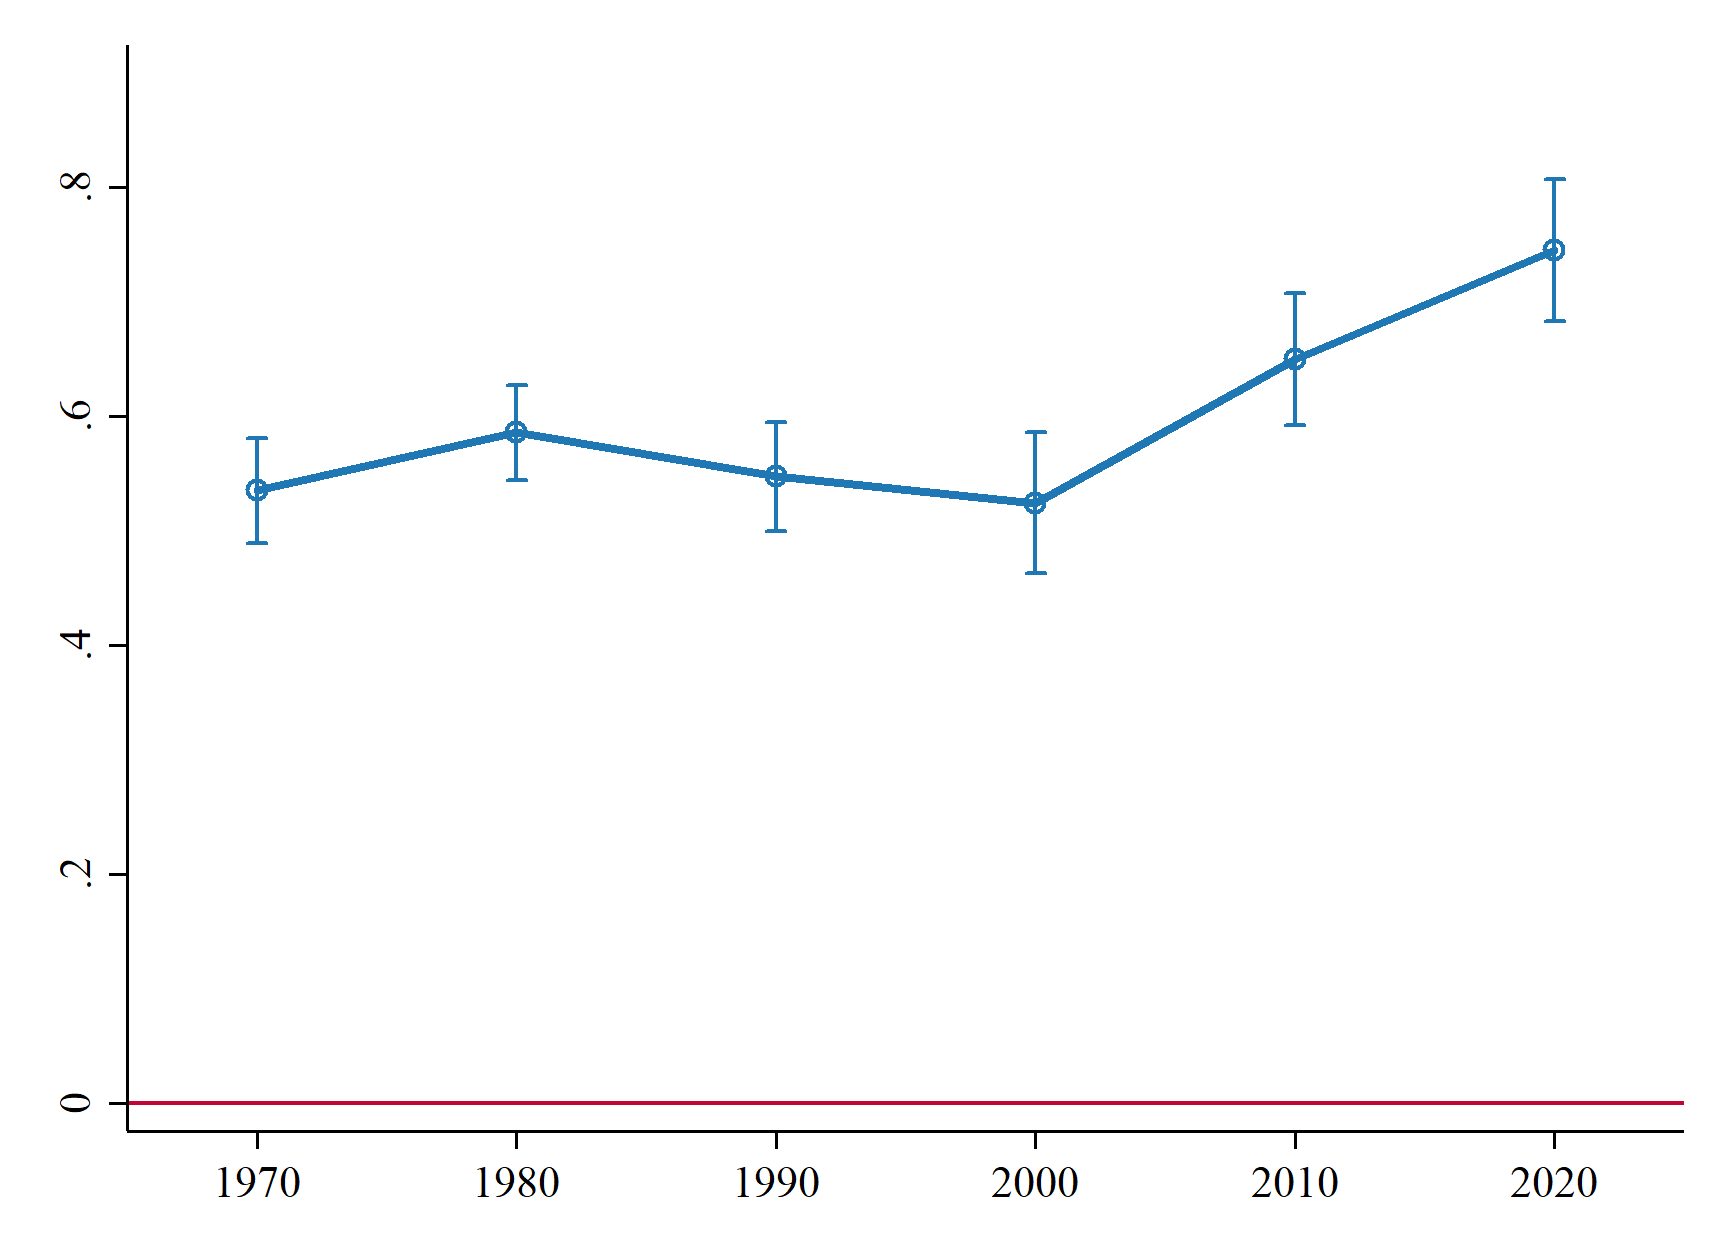
\includegraphics[width=.5\textwidth]{../2_analysis/output/figures/high_wage_ind_men}} \subfloat[Women's high-wage industry employment]{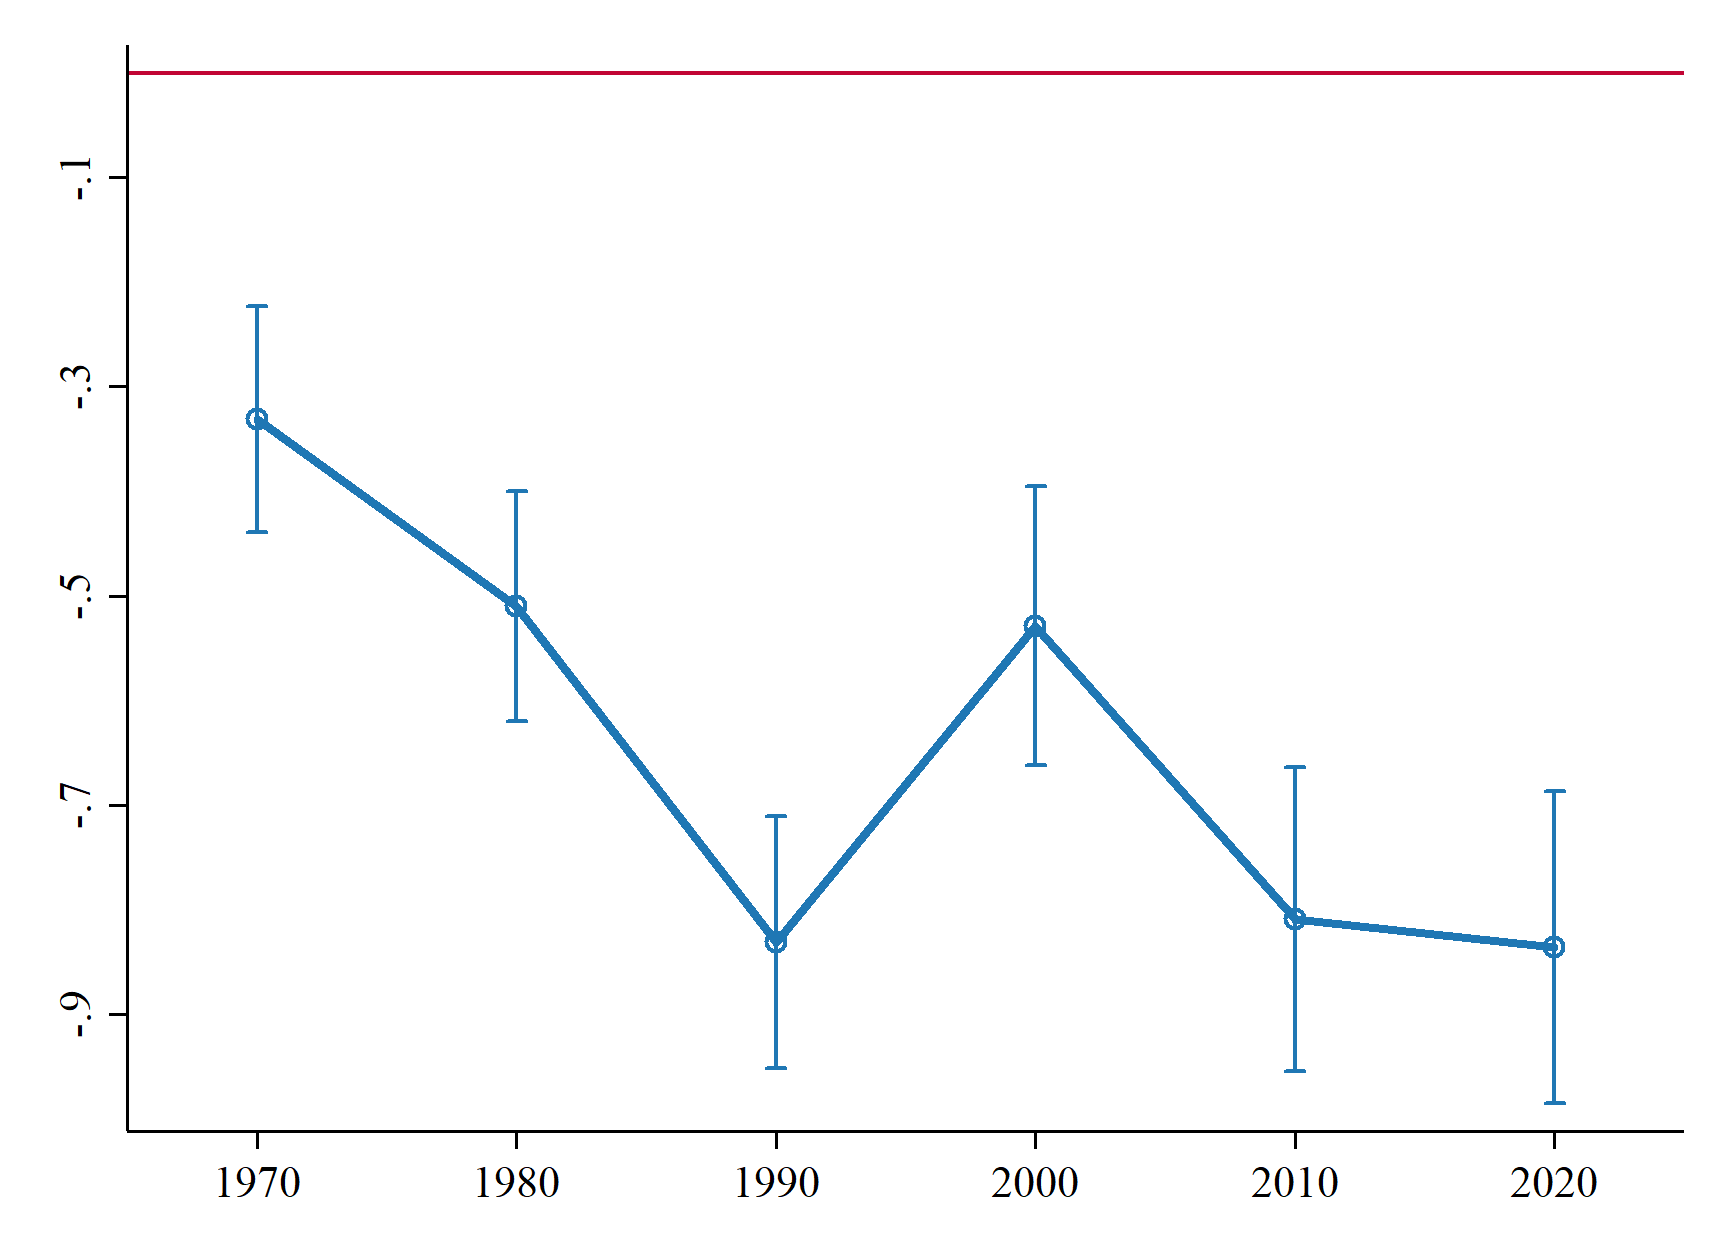
\includegraphics[width=.5\textwidth]{../2_analysis/output/figures/high_wage_ind_women}} \\ 
\par \begin{minipage}[h]{\textwidth}{\tiny\textbf{Note:} figure restricts to CZ with more than 1 people per km$^2$. Figure generated on 30 Nov 2020 at 18:49:34.}\end{minipage}
\end{figure}


\subsubsection{Is this about decline of these industries, or women's access to these coveted jobs?}
Consider the following regression:
\beqns
gap_{rt}=\alpha_t+\beta_{t}\ln(density)_{rt}+\chi_ts_{rt}^{highpay}+\delta_t{male\_share}_{rt}^{highpay,f}
\eeqns
The idea here is to distinguish between two possible stories:
\bitem
	\item \textbf{Decline of high pay industries:} men in cities are heavily concentrated in industries that in urban decline.
	\item \textbf{Women access to better employment:} women in cities are initially excluded from high-pay jobs. Over time, they are able to access to these high-pay, which looks like a gain relative to men.
\eitem

\subsubsection{High pay industries are mostly manufacturing industries. Is 1970-1990 this about manufacturing?}


No. Suppose the story at work here is:
\bitem
	\item Manufacturing is concentrated in cities.
	\item Manufacturing is heavily male and high-pay.
	\item Over time, women get access to these coveted jobs.
\eitem

Then, this could be captured in the regression,
\beqns
	gap_{rt}=\alpha_t+\beta_{t}\ln(density)_{rt}+\chi_ts_{rt}^{manufacturing}
\eeqns
where we should expect the density gradient to disappear during 1970-1990. This is not what figure shows \ref{fig:manufacturing_gradients}. Thus the point has to be more subtle.

\begin{figure}[!h]
\centering
\caption{High wage industries by gender}
\label{fig:manufacturing_gradients}
\subfloat[Net-of race/age gender gap and high-wage industry share]{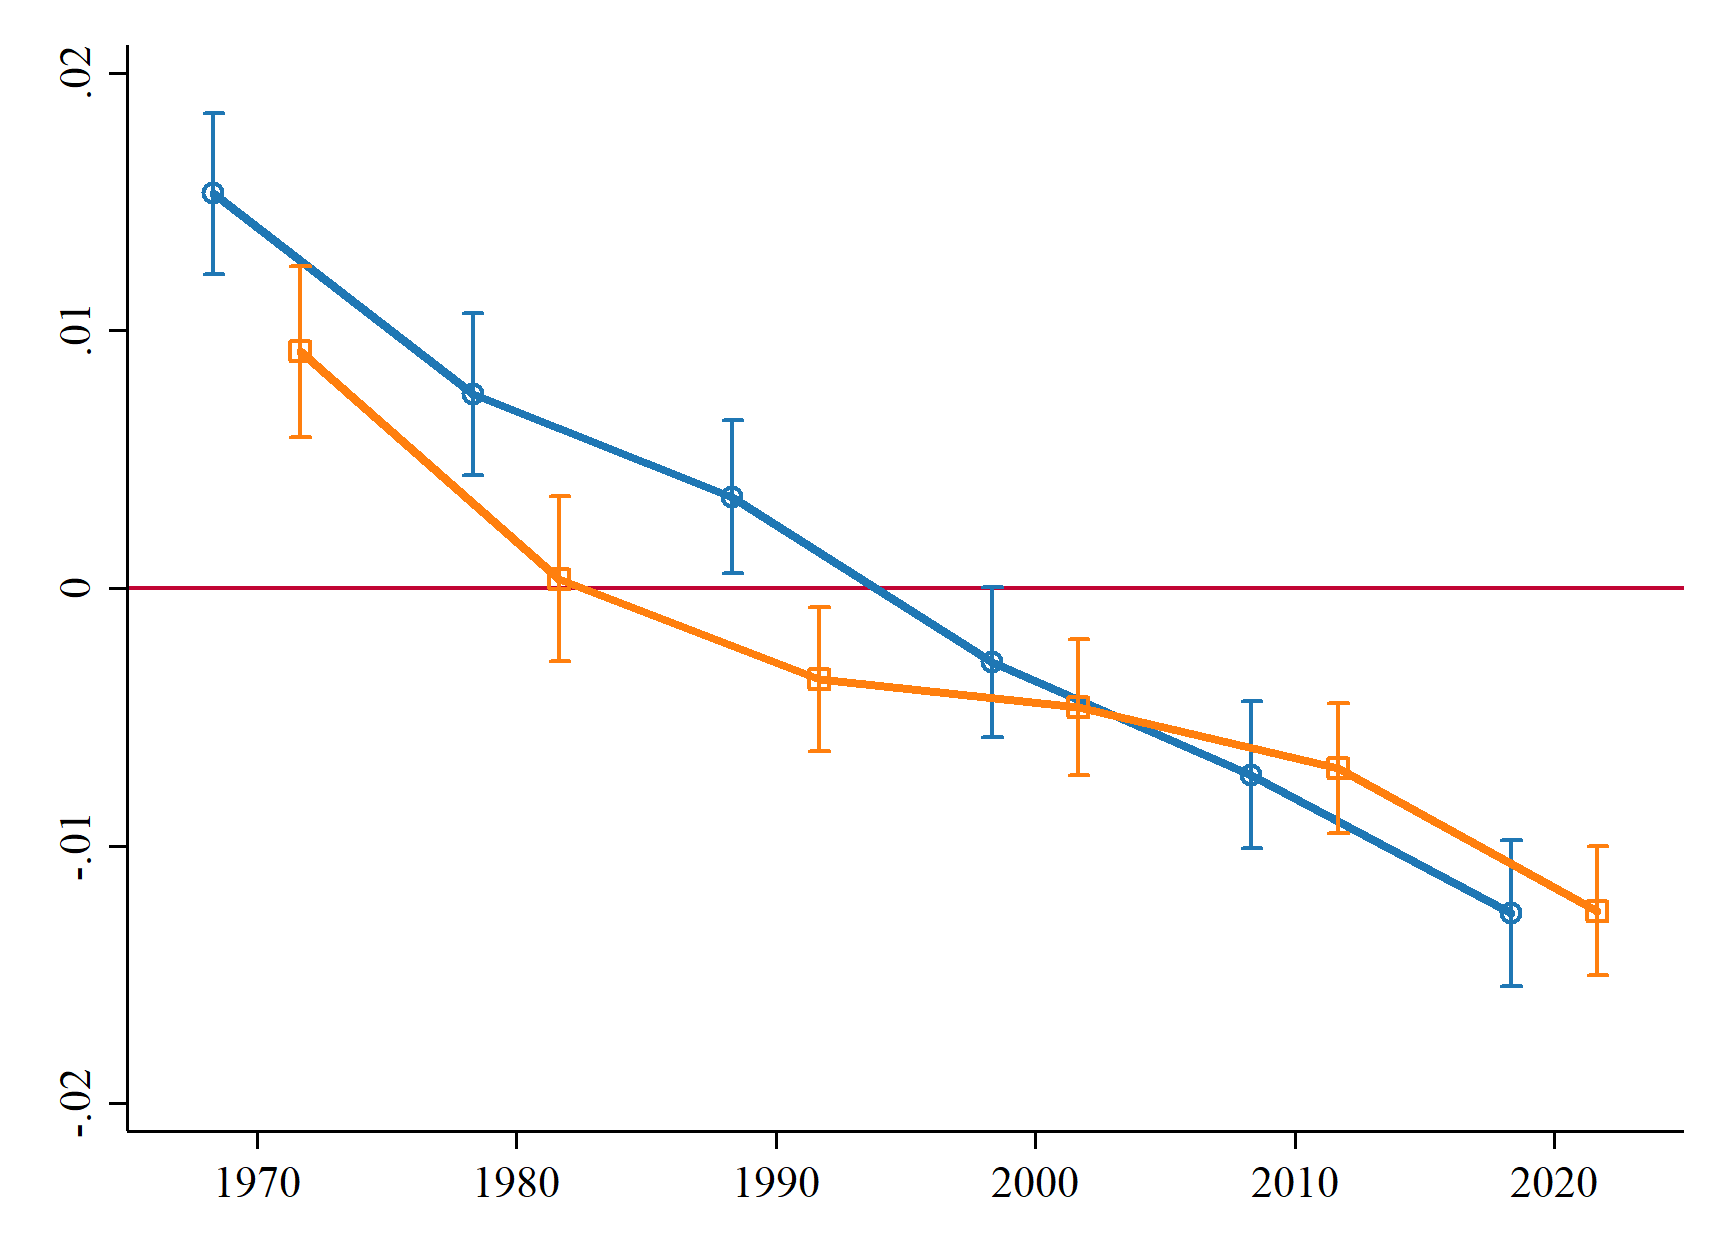
\includegraphics[width=.5\textwidth]{../2_analysis/output/figures/gender_bas_gap_gradient_manufacturing_share}} \subfloat[Net-of-education gap and high-wage industry share]{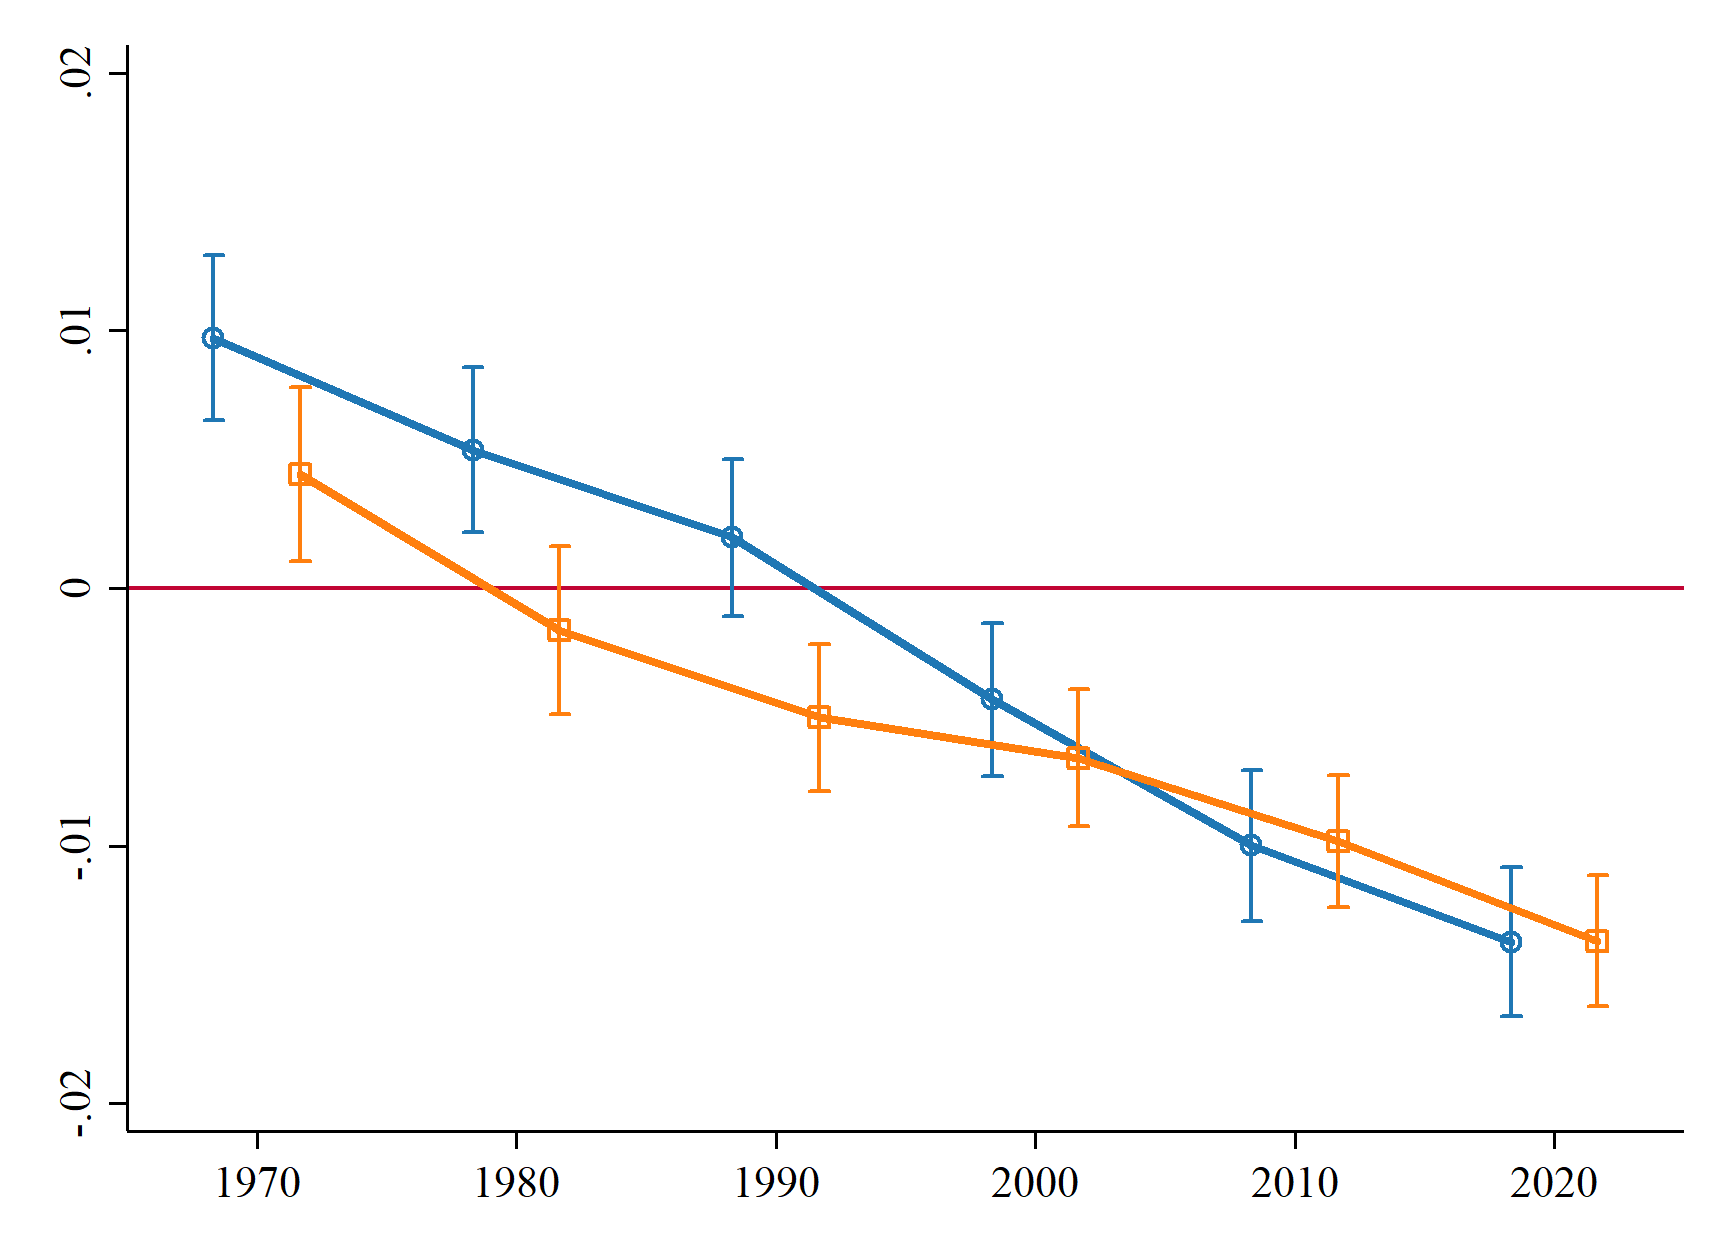
\includegraphics[width=.5\textwidth]{../2_analysis/output/figures/gender_hum_gap_gradient_manufacturing_share}} \\ 
\par \begin{minipage}[h]{\textwidth}{\tiny\textbf{Note:} figure restricts to CZ with more than 1 people per km$^2$. Figure generated on 30 Nov 2020 at 18:49:36.}\end{minipage}
\end{figure}



\subsubsection{What is different about the high-pay industries?}



\subsubsection{Why doesn't industry account for the drift after 1990?}

Following evidence presented in \ref{fig:ind_cities} the gradient on high-pay industries essentially disappears $\implies$ CZ-industry specialization stops driving the gradient.

It would also be hart to argue that gender differences  across 

\begin{figure}[!h]
\centering
\caption{High wage industries by gender}
\label{fig:gender_ind_cities}
\subfloat[Variable industry ranking]{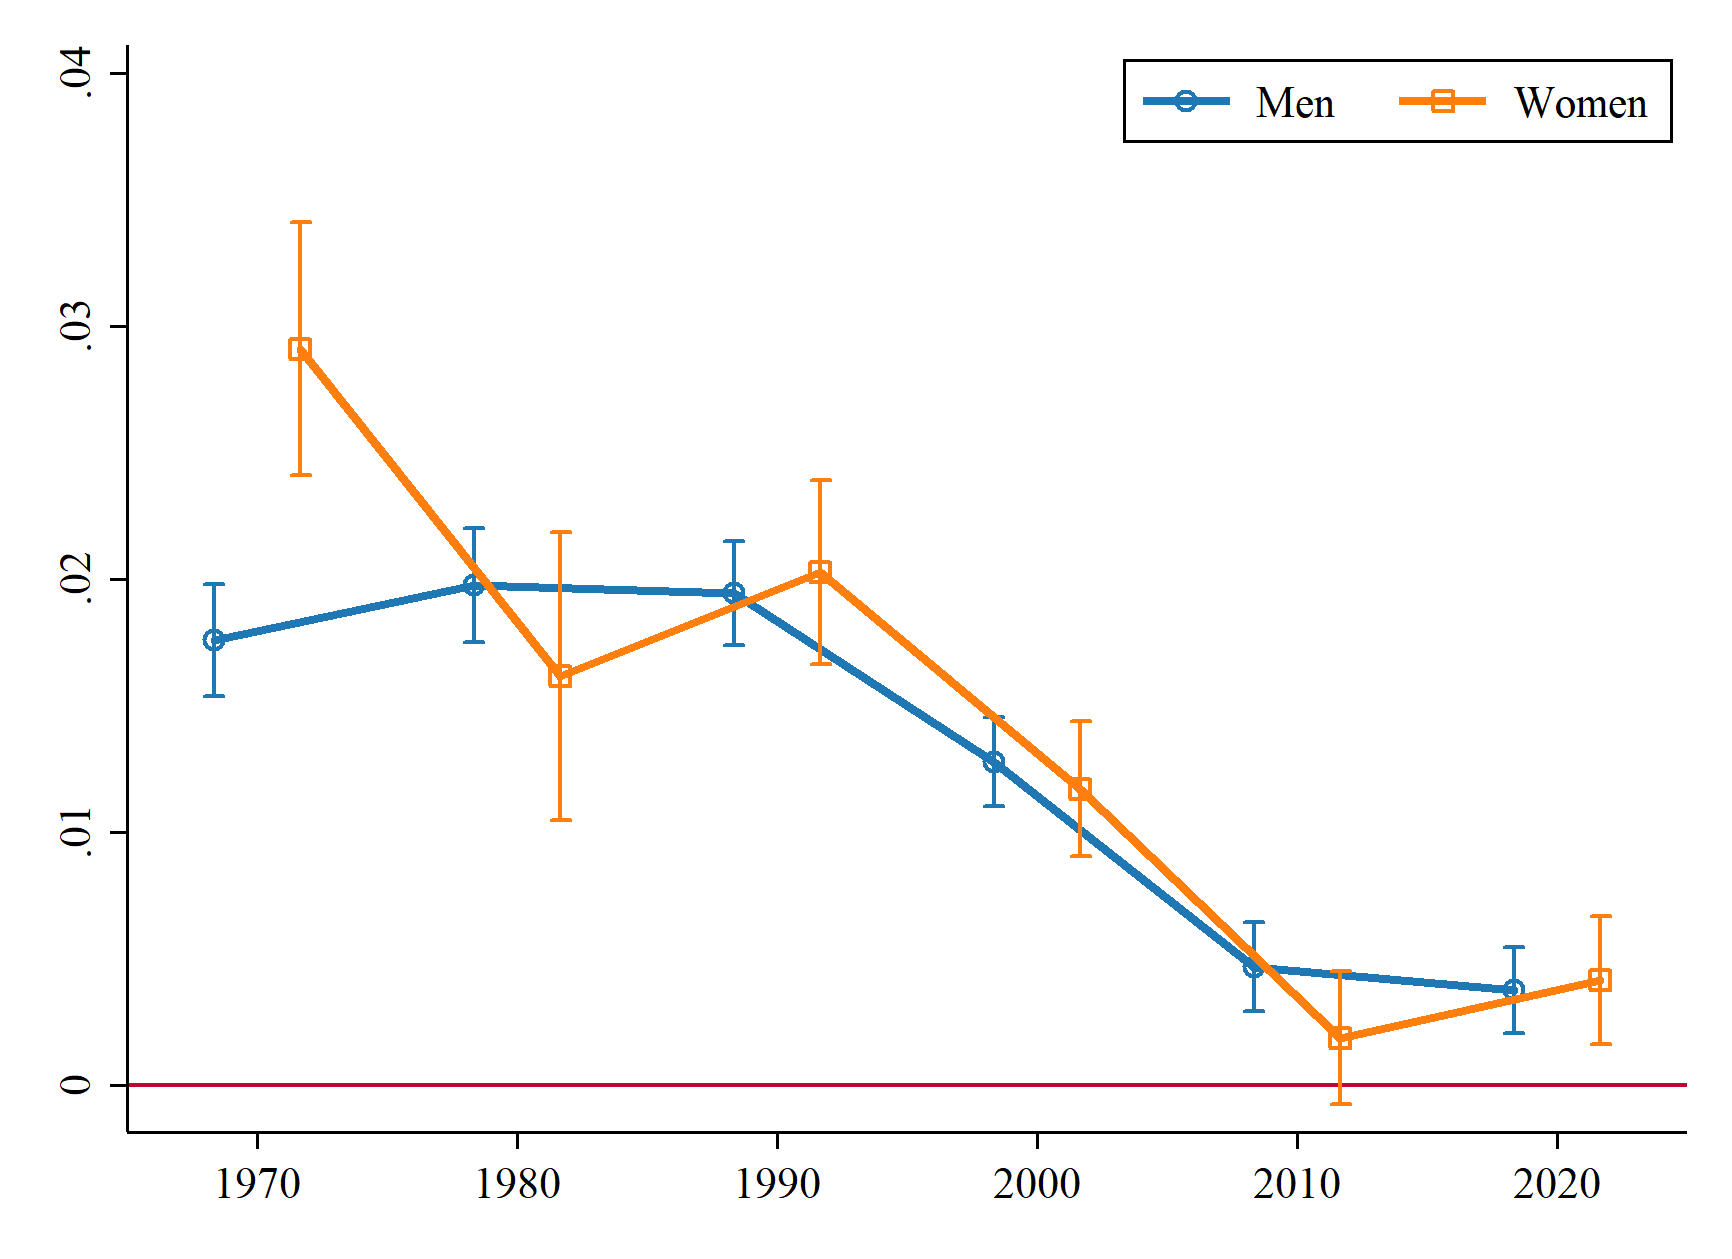
\includegraphics[width=.5\textwidth]{../2_analysis/output/figures/high_pay_gender_gradient}} \subfloat[Industry ranking fixed at 1970]{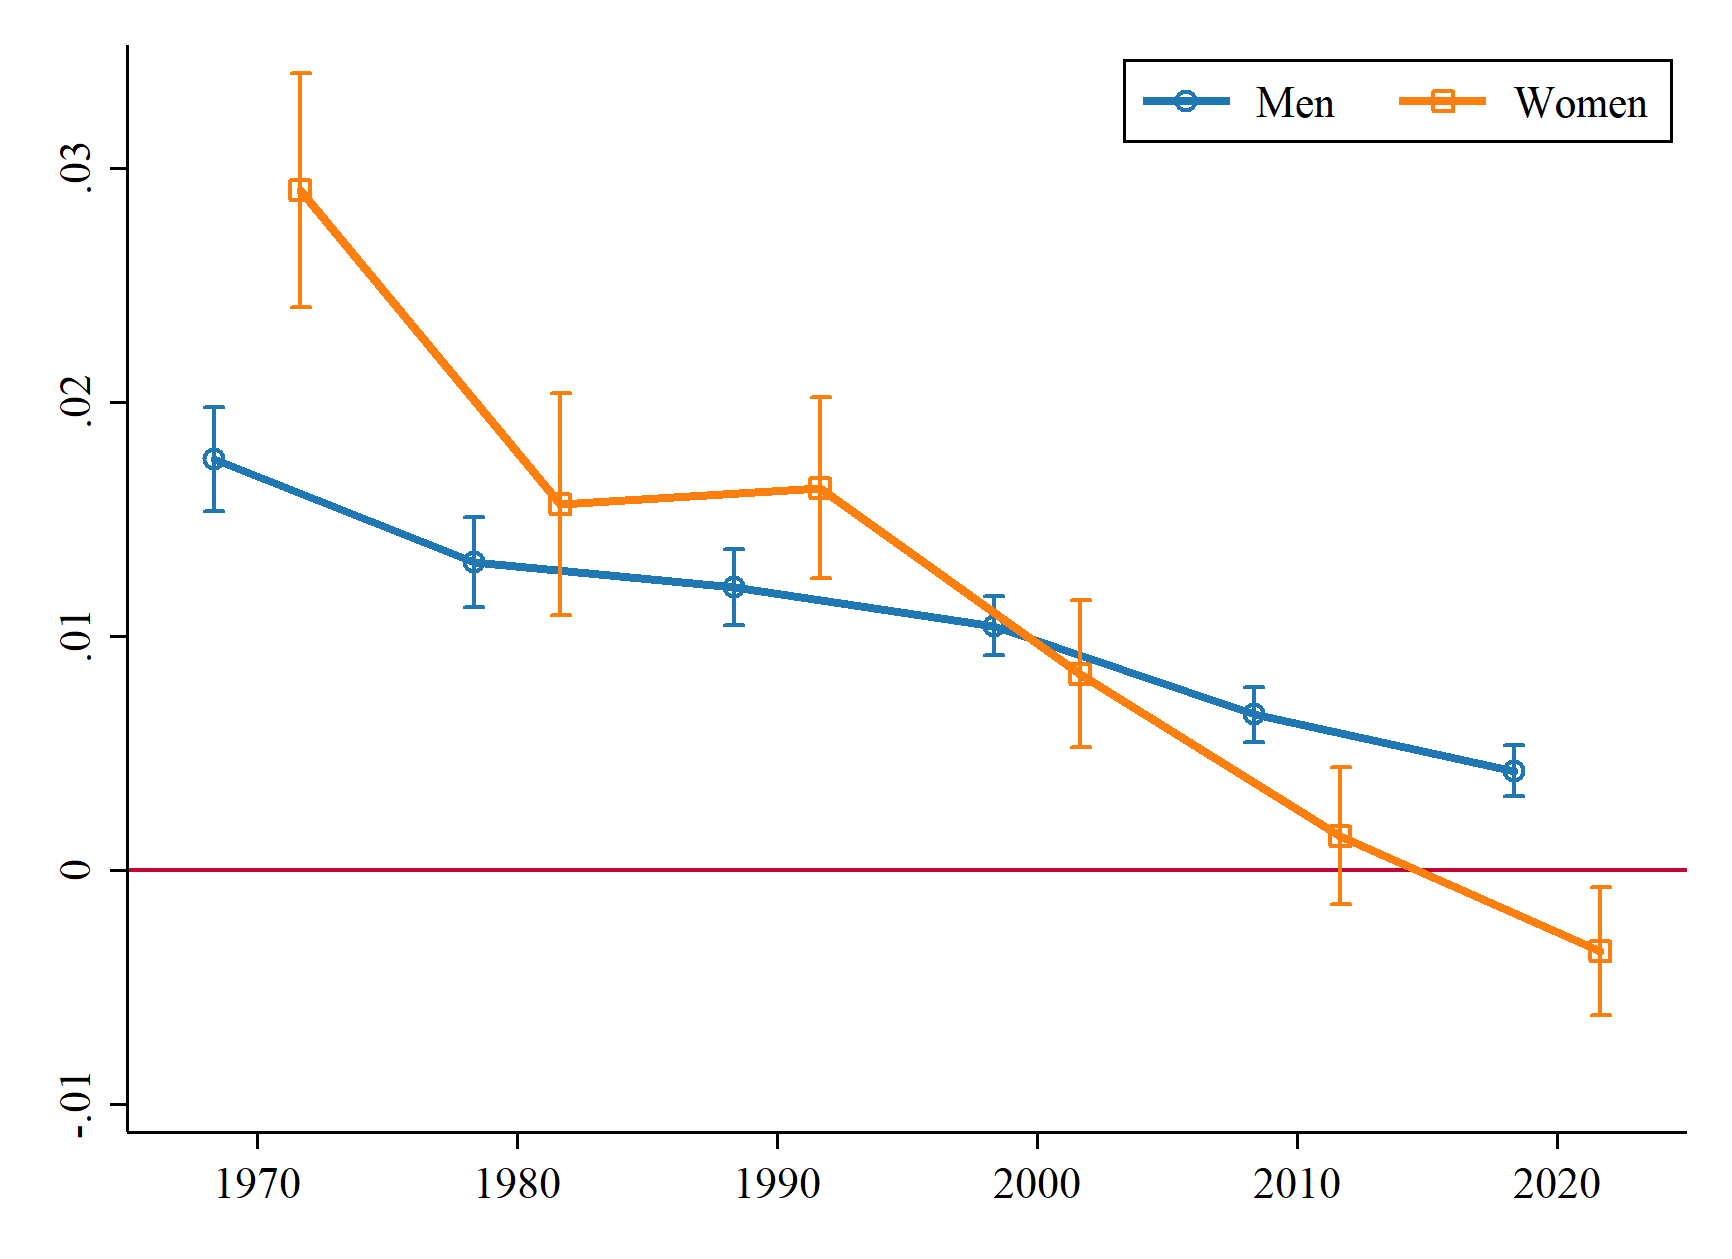
\includegraphics[width=.5\textwidth]{../2_analysis/output/figures/high_pay_gender_gradient_70}} \\ 
\par \begin{minipage}[h]{\textwidth}{\tiny\textbf{Note:} figure restricts to CZ with more than 1 people per km$^2$. Figure generated on 30 Nov 2020 at 23:02:04.}\end{minipage}
\end{figure}



\subsubsection{Taking stock:}
\textbf{Explaining the positive gradient during 1970-1990}
\bitem
	\item High-pay industries were heavily concentrated in dense commuting zones.
	\item These high pay industries (mostly manufacturing) where heavily male.
	\item The two above facts $\implies$ women were less likely to have high pay in densest cities $\implies$ positive gender-gap gradient over 1970-1990.
\eitem
\bitem
	\item Over time, high-pay industries become more service intensive. Services more female-friendly industries $\implies$ there's little difference in the employment distribution 
	\item Moreover, industries (such as manufacturing) are in fast decline in the densest labor markets.
\eitem
So, overall I think that 1970-1990 can be explained by decline in manufacturing. Whatever is happening from 1990 cannot be explained by manufacturing decline. Gradient in manufacturing is likely flat by the end of the period.	

[next step$=>$ what happens if I just control for the share of manufacturing in the aggregate level regression]

[structural transformation was larger in denser cities $\implies$ change towards female driven industries]

[Story after the 1990s appear to be more complicated]